%%%%%%%%%%%%%%%%%%%%%%%%%%%%%%%%%%%%%%%%%%%%%%%%%%%%%%%%%%%%%%%%%%%%%%%%%%%%%%%%
%2345678901234567890123456789012345678901234567890123456789012345678901234567890
%        1         2         3         4         5         6         7         8

\documentclass[letterpaper, 10 pt, conference]{ieeeconf}  % Comment this line out if you need a4paper

%\documentclass[a4paper, 10pt, conference]{ieeeconf}      % Use this line for a4 paper

\IEEEoverridecommandlockouts                              % This command is only needed if 
                                                          % you want to use the \thanks command

\overrideIEEEmargins                                      % Needed to meet printer requirements.

% See the \addtolength command later in the file to balance the column lengths
% on the last page of the document

\makeatletter
\let\NAT@parse\undefined
\makeatother

\usepackage{xspace}
\usepackage{amsmath,amssymb,amsfonts,amsfonts}
\usepackage{algorithm}
\usepackage[noend]{algorithmic}
\usepackage{url}
\usepackage{bm}
\usepackage{graphicx}
\usepackage[font=footnotesize]{caption} % incompatible with aaai.sty?
\usepackage[font=footnotesize]{subcaption}
\usepackage{color}
\usepackage{cite}
\usepackage{hyperref}
\usepackage{eqparbox}
%\hypersetup{bookmarksopen,
%bookmarksnumbered,
%pdfpagemode=UseOutlines,
%colorlinks=true,
%linkcolor=blue,
%anchorcolor=blue,
%citecolor=blue,
%filecolor=blue,
%menucolor=blue,
%urlcolor=blue
%}


\title{\LARGE \bf
Generalizing Informed Sampling
for Asymptotically Optimal Sampling-based Planning via Markov Chain
Monte Carlo Methods
}


\author{
Daqing Yi$^{*}$,
Rohan Thakker$^{*}$,
Oren Salzman$^{}$,
Cole Gulino$^{}$ and
Siddhartha Srinivasa$^{}$% <-this % stops a space
\thanks{*Daqing Yi and R. Thakker contributed equally to this paper.}
\thanks{This work was (partially) funded by the National Science Foundation IIS (\#1409003), Toyota Motor Engineering \& Manufacturing (TEMA), and the Office of Naval Research.}% <-this % stops a space
\thanks{$^{1}${\tt\small \{rthakker, cgulino, daqingy, osalzman, ss5\} @andrew.cmu.edu}}%
%
\\        
Robotics Institute, Carnegie Mellon University$^{1}$
}

%%%%%%%%%%%%%%%%%%%%%%%%%%%%%%%%%%%%%%%%%%%%%%%%%%%%%%%%%%%%%%%%%%%%%%%%%%%%%%
%  macros 
%%%%%%%%%%%%%%%%%%%%%%%%%%%%%%%%%%%%%%%%%%%%%%%%%%%%%%%%%%%%%%%%%%%%%%%%%%%%%%

% Caligraphic letters:
\newcommand{\calA}{\ensuremath{\mathcal{A}}\xspace}
\newcommand{\calC}{\ensuremath{\mathcal{C}}\xspace}
\newcommand{\calE}{\ensuremath{\mathcal{E}}\xspace}
\newcommand{\calG}{\ensuremath{\mathcal{G}}\xspace}
\newcommand{\calR}{\ensuremath{\mathcal{R}}\xspace}
\newcommand{\calM}{\ensuremath{\mathcal{M}}\xspace}
\newcommand{\calX}{\ensuremath{\mathcal{X}}\xspace}
\newcommand{\calS}{\ensuremath{\mathcal{S}}\xspace}
\newcommand{\calQ}{\ensuremath{\mathcal{Q}}\xspace}
\newcommand{\calT}{\ensuremath{\mathcal{T}}\xspace}
\newcommand{\calL}{\ensuremath{\mathcal{L}}\xspace}
\newcommand{\calB}{\ensuremath{\mathcal{B}}\xspace}
\newcommand{\calO}{\ensuremath{\mathcal{O}}\xspace}
\newcommand{\calP}{\ensuremath{\mathcal{P}}\xspace}
\newcommand{\calU}{\ensuremath{\mathcal{U}}\xspace}

% math
\newcommand{\R}{\mathbb{R}}
\newcommand{\Z}{\mathbb{Z}}
\newcommand{\A}{\mathbb{A}}
\newcommand{\N}{\mathbb{N}}
\newcommand{\Q}{\mathbb{Q}}
\newcommand{\C}{\mathbb{C}}
\newcommand{\K}{\mathbb{K}}
\newcommand{\D}{\mathbb{D}}


% Motion planning
\newcommand{\Cfree}{\ensuremath{\calX_{\rm free}}\xspace}
\newcommand{\Cforb}{\ensuremath{\calX_{\rm obs}}\xspace}
%\newcommand{\Cinf}{\ensuremath{\calX_{\hat{f}}}\xspace}
\newcommand{\Cinf}{\ensuremath{\calX_{\rm {inf}}}\xspace}
\newcommand{\Ufree}{\ensuremath{\calU_{\rm free}}\xspace}
\newcommand{\Pinf}{\ensuremath{\pi_{\hat{f}}}\xspace}


\newcommand{\Cbest}{\ensuremath{c_{\rm{curr}}}\xspace}

\newcommand{\Cs}{C-space\xspace}
\newcommand{\Css}{C-spaces\xspace}

\newcommand{\DOF}{\textit{dof}\xspace}
\newcommand{\DOFs}{\textit{dofs}\xspace}

\newcommand{\cbest}{\ensuremath{c_{\rm best}}\xspace}

% =
\newcommand{\eg}{{e.g.}\xspace}
\newcommand{\ie}{{i.e.}\xspace}
\newcommand{\etc}{{etc.}\xspace}
\newcommand{\etal}{{et~al.}\xspace}

\def\naive{{na\"{\i}ve}\xspace}

\def\os#1{\textcolor{magenta}{#1}}
\def\dy#1{\textcolor{cyan}{#1}}
\def\rt#1{\textcolor{green}{#1}}
\def\cg#1{\textcolor{blue}{#1}}
\def\ss#1{\textcolor{red}{#1}}

\def\deprecated#1{\vspace{3mm} \textcolor{red}{#1}  \vspace{3mm}}


\newtheorem{thm}{Theorem}
\newtheorem{lem}{Lemma}
\newtheorem{defn}{Definition}
%\newtheorem{thm}{Theorem}[section]
\newtheorem{observation}[thm]{Observation}
%\newtheorem{thm}{Theorem}
%\newtheorem{cor}[thm]{Corollary}
%\newtheorem{lem}[thm]{Lemma}


%tex tools
\newcommand{\ignore}[1]{}
\newcommand{\first}[2]{#1}
\newcommand{\second}[2]{#2}
\newcommand{\arxiv}[2]{#2}



\newcommand{\captionstyle}{\sf \footnotesize }

\renewcommand\algorithmiccomment[1]{%
  \hfill\#\ \eqparbox{COMMENT}{#1}%
}

\begin{document}

\maketitle
\thispagestyle{empty}
\pagestyle{empty}


%%%%%%%%%%%%%%%%%%%%%%%%%%%%%%%%%%%%%%%%%%%%%%%%%%%%%%%%%%%%%%%%%%%%%%%%%%%%%%%%
\begin{abstract}

\end{abstract}


%%%%%%%%%%%%%%%%%%%%%%%%%%%%%%%%%%%%%%%%%%%%%%%%%%%%%%%%%%%%%%%%%%%%%%%%%%%%%%%%
\section{Introduction}
\label{sec:intro}


Sampling-based motion-planning algorithms~\cite{CBHKKLT05, L06} have proven to be an effective tool at solving motion-planning problems.
They search through a continuous state space~$\calX$ by sampling random states and maintaining a discrete graph~$G$ called a \emph{roadmap}.
Vertices and edges in $G$ correspond to collision-free states and paths, respectively.

Roughly speaking, these algorithms iteratively sample new states.
This is required to ensure that, as the number of samples tends to infinity, 
(i)~a solution will be found 
%(a property called \emph{probabilistic completeness})
and that
(ii)~given some optimization criteria, the quality of the solution will progressively converge to the quality of the optimal solution.
%(a property called \emph{asymptotic  optimality}).

Initially, 
when a path has yet to be found, 
the samples are drawn from the entire state space~$\calX$.
However, once a path $\gamma$ is produced,  algorithms that seek \emph{high-quality paths} can limit their sampling domain to a subset of~$\calX$ only  containing states that may be used to produce higher-quality paths than~$\gamma$.
Following Gammell et al.~\cite{GSB14}, we call this subset the \emph{informed subset} and denote it~$\Cinf$.
In this work we address the problem of efficiently producing samples in informed subset for systems with arbitrary complex costs. 

For Euclidean spaces optimizing for path length, 
\Cinf can be analytically expressed as a prolate hyperspheroid and can be sampled directly using a closed-form solution~\cite{GSB14}.
Indeed, directly sampling in \Cinf has been shown to dramatically improve computation time when compared to sampling in~$\calX$, especially in high dimensions. 

Unfortunately, in more general settings,
it is not clear how to directly sample \Cinf.
%
One approach to produce samples in~\Cinf is via \emph{rejection sampling}---sampling a state $x \in \calX$ and testing if $x \in \Cinf$.
However, when the size of the informed space~$\Cinf$ is much smaller than entire state space~$\calX$, this procedure is highly inefficient, dominating the running time of the algorithm~\cite{KTC16}.
Recently, Kunz et al.~\cite{KTC16} showed, under some technical assumptions, how to partially ameliorate this inefficiently by \emph{Hierarchical rejection sampling} (HRS). 
Here, individual dimensions are sampled recursively 
and then combined. Rejection sampling is performed for these partial samples until a suitable sample has been produced. 
%The novelty of HRS is the ability to fail fast. 
Unfortunately, HRS may still produce a large number of rejected samples especially in high-dimensional spaces~\cite{KTC16}.
This may cause the planning algorithm to spend most of its time trying to produces samples in~$\Cinf$ rather than explore it.

\begin{figure}[tb]
  \centering
  	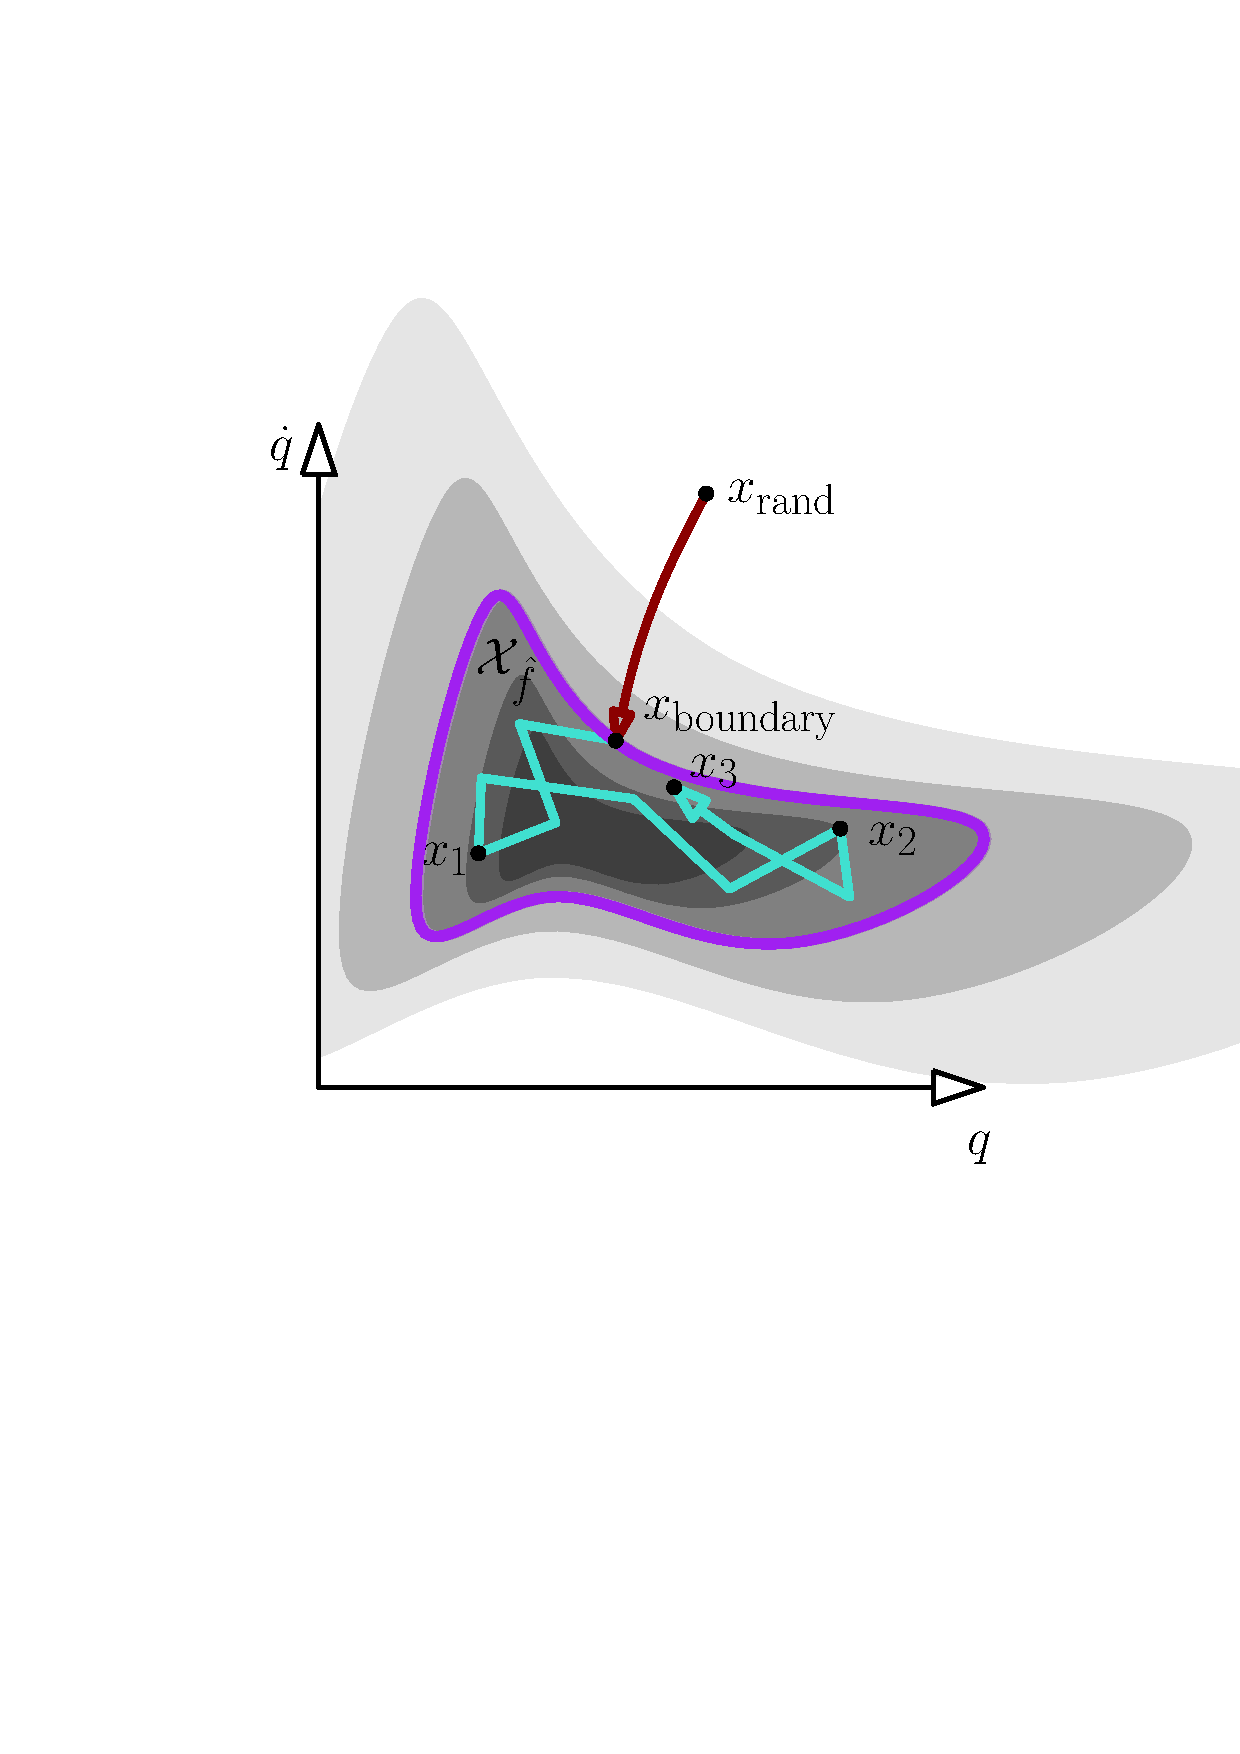
\includegraphics[trim={4.5cm 0 4cm 2cm},clip,height = 5.25cm ]{fig/alg.pdf}
  \caption{
    \captionstyle
  	Algorithmic approach.
  	Cost function is depicted using isocontours (darker shades reflect lower cost) while the boundary of the informed set is depicted in purple. 
  	The root-finding and MCMC algorithms are depicted in blue and green, respectively.
  	}
   	\label{fig:alg}
\end{figure}


In this paper, we suggest an alternative approach to produce samples in the informed set \Cinf for a wide range of settings.
\textbf{
Our main insight is to recast this problem as one of sampling uniformly within a level set of an implicit function.
This recasting enables us to apply Monte Carlo sampling methods, used very effectively in the Machine Learning and Optimization communities, to solve our problem.
}
Specifically, our approach, depicted in Fig~\ref{fig:alg} consists of two stages:
in the first, a random sample $x \in \calX$ is retracted to the boundary of~$\Cinf$ by running a root-finding algorithm;
in the second stage, this retracted sample  is used to seed a Monte Carlo sampling chain which allows us to  produce samples that (approximately) cover~$\Cinf$  uniformly.

While our approach can be used with any Markov chain Monte Carlo (MCMC) method, it is especially suited to be used with hit and run~\cite{S84,KSZ11}.
Roughly speaking, this is because hit and run (detailed in Sec~\ref{sec:related_work})
performs a series of one-dimensional rejection samples which are extremely fast to compute, even in high-dimensional spaces. 

Our approach requires that the system has a solution to the two-point boundary value problem (2pBVP)~\cite{L06, H02} and that a gradient can be defined over the cost function.
Indeed, we demonstrate the efficiency of our approach on a wide variety of systems and show that it enables reducing the planning time by several orders of magnitude when compared to algorithms using rejection sampling or HRS.

\begin{figure*}[t!]
	\centering
	\begin{subfigure}[b]{\textwidth}
		\centering
		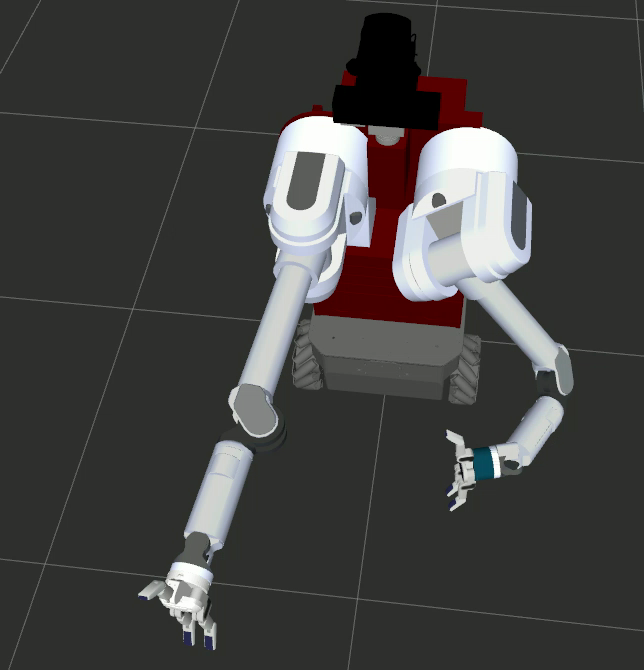
\includegraphics[height=3cm]{fig/motivation/slow1}
		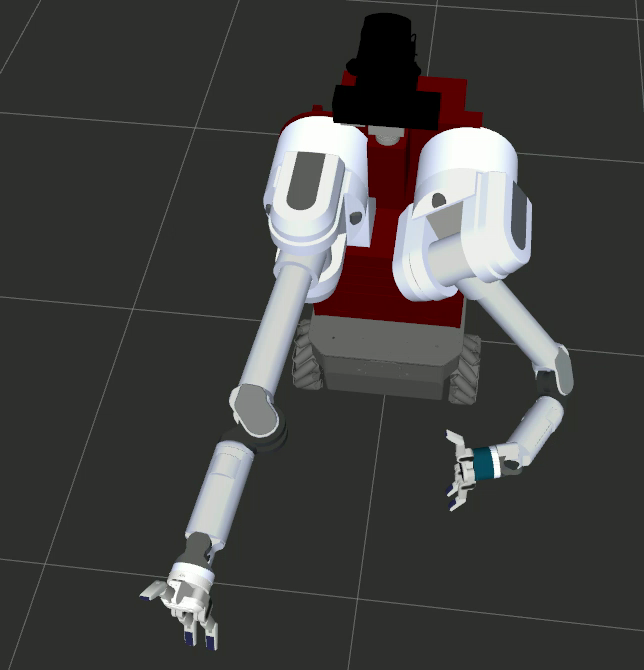
\includegraphics[height=3cm]{fig/motivation/slow2}
		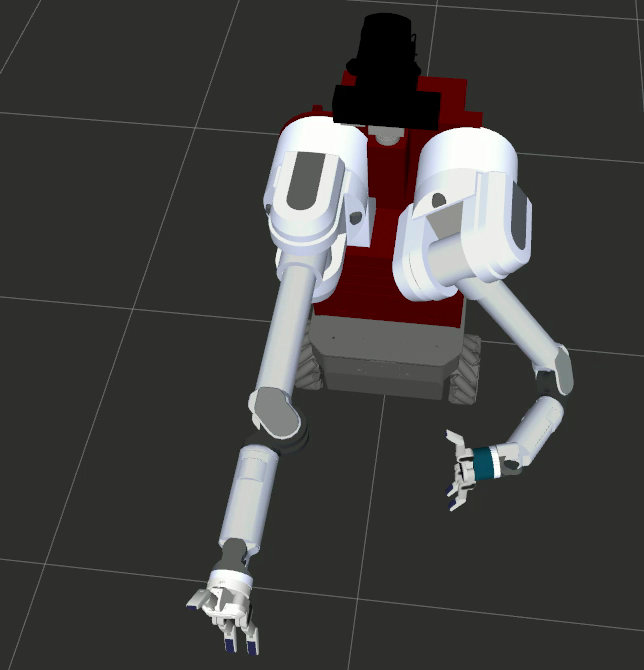
\includegraphics[height=3cm]{fig/motivation/slow3}
		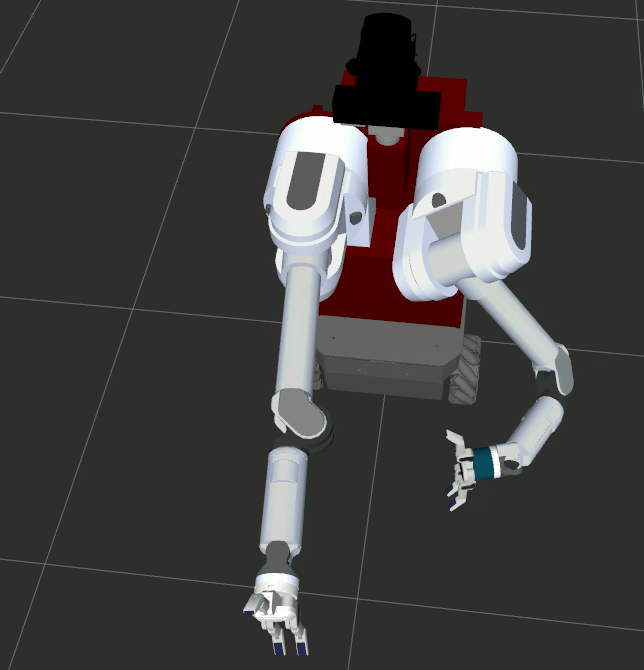
\includegraphics[height=3cm]{fig/motivation/slow4}
		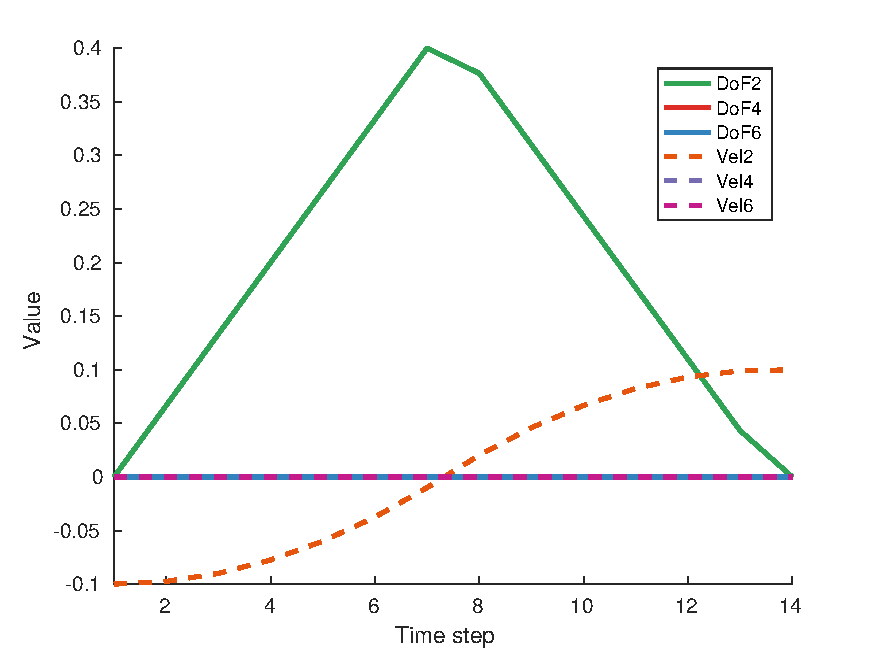
\includegraphics[height=3cm]{fig/motivation/slowmotion}
		\caption{Zero goal velocity}
		\label{fig:motivation:slow}
	\end{subfigure}
	\begin{subfigure}[b]{\textwidth}
		\centering
		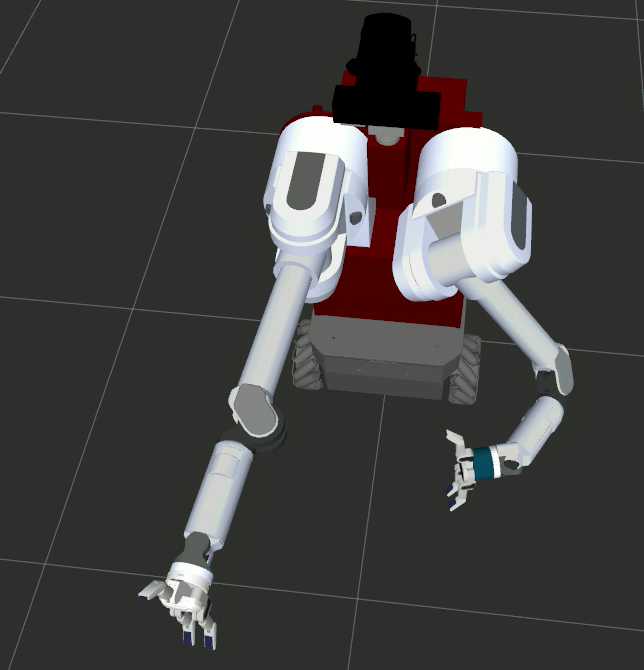
\includegraphics[height=3cm]{fig/motivation/fast1}
		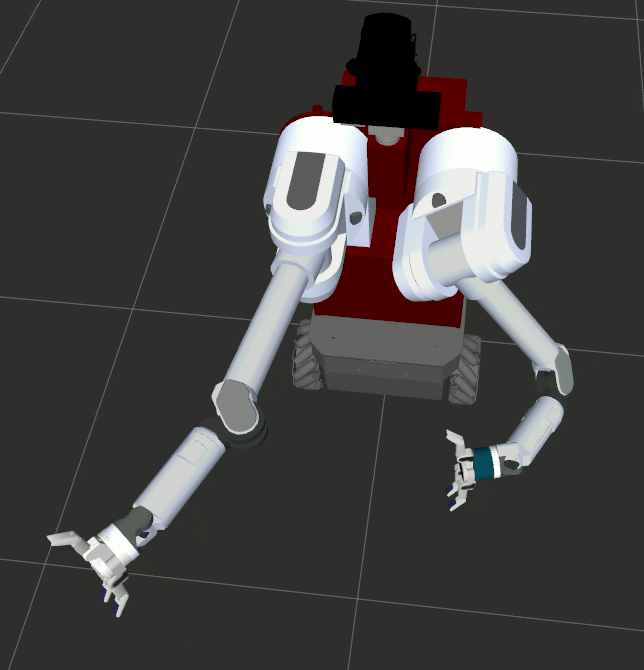
\includegraphics[height=3cm]{fig/motivation/fast2}
		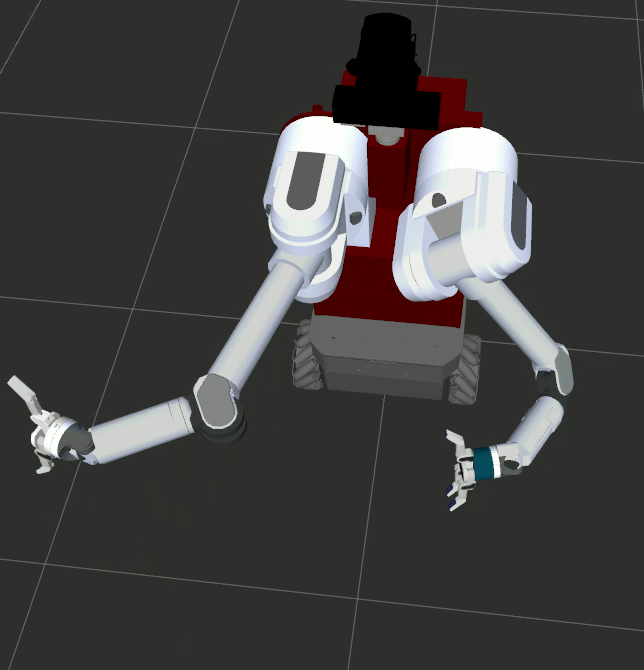
\includegraphics[height=3cm]{fig/motivation/fast3}
		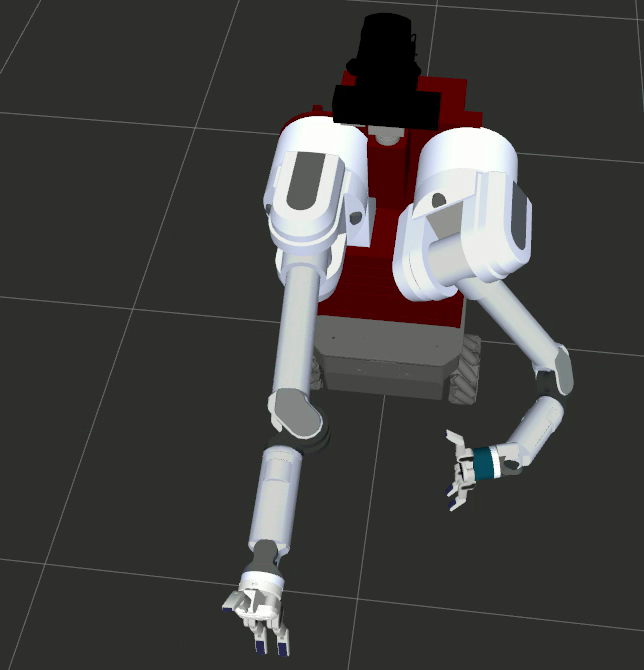
\includegraphics[height=3cm]{fig/motivation/fast4}
		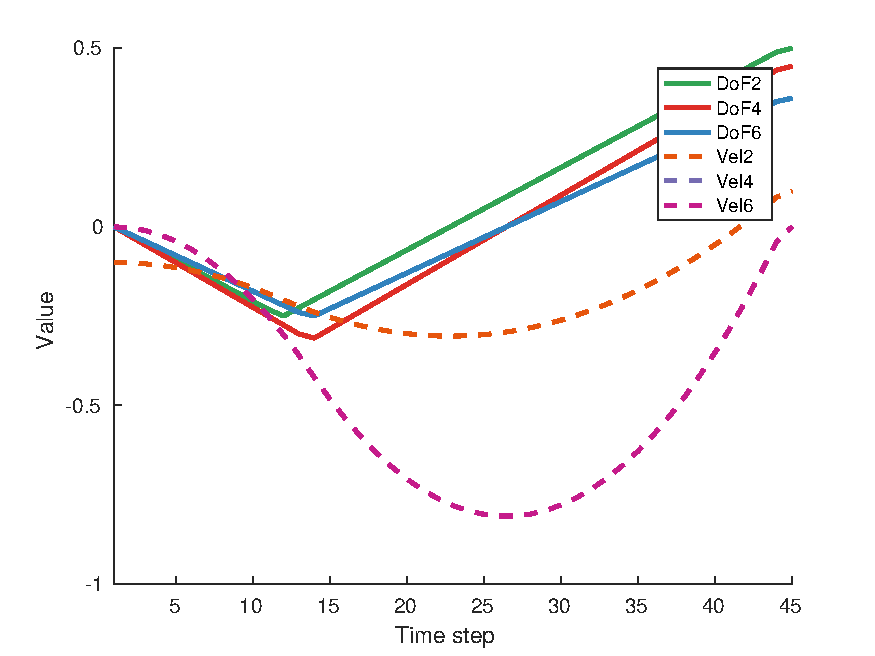
\includegraphics[height=3cm]{fig/motivation/fastmotion}
		\caption{Non-zero goal velocity}
		\label{fig:motivation:fast}
	\end{subfigure}
	\caption{HERB moves right arm from a start configuration to a goal configuration, which are very close.
    When the goal velocity is non-zero, HERB needs to move right arm further away to accelerate.
	}
	\label{fig:motivation}
\end{figure*} 

\os{structure}

\section{Related work}
\label{sec:related_work}
We start in Sec.~\ref{subsec:planning} by giving an overview of relevant sampling-based motion-planning algorithms.
We then continue in Sec.~\ref{subsec:sampling} to describe different approaches that can be used by  these algorithms to sample~$\calX$.
We conclude our literature review in Sec.~\ref{subsec:mcmc} with a brief overview of Markov Chain Monte Carlo methods.

\subsection{Sampling-based motion-planning algorithms}
\label{subsec:planning}
Initial sampling-based algorithms such as RRT~\cite{LK01} and PRM~\cite{KSLO96} did not take into account the \emph{quality} of a path, given some optimization criteria, and only guaranteed to asymptotically return \emph{a} solution, if one exists.
Karaman and Frazzoli~\cite{KF11}, presented variants of PRM and RRT, named PRM* and RRT*, respectively that were shown to produce paths who's cost converges asymptotically to the minimal-cost path.
This was done by recognizing the underlying connections between stochastic sampling-based motion planning and the theory of random geometric graphs (see also~\cite{SSH16}).
Additional algorithms followed, increasing the converges rate by various techniques such as 
lazy dynamic programming~\cite{GSB15, JSCP15, SH15},
relaxing optimality to near-optimality~\cite{DB14, SH16} 
and more.


Many of the algorithms mentioned require solving a two-point boundary value problem (2pBVP) to perform exact and optimal connections between vertices in the roadmap.
For holonomic robots, these are simply straight lines in the configuration space, but for kinodynamic sytems with arbitrary cost functions,  computing an optimal trajectory between two states is non-trivial in general.

Xie et al.~\cite{XBPA15} use a variant of sequential quadratic programming (SQP) to solve 2pBVP and integrate it with BIT*~\cite{GSB15}.
Webb and van den Berg~\cite{WB13} use a fixed-final-state-free-final-time controller to solve the 2pBVP  with respect to a cost function that allows for balancing between the duration of the trajectory and the expended control effort.
Perez et al.~\cite{PPKKL12} propose a variant of RRT* that automatically defines a distance metric and node extension method by locally linearizing
the domain dynamics and applying linear quadratic regulation (LQR).

Finally, we note that we are not the first to integrate Monte Carlo sampling into planning algorithms. T-RRT~\cite{JCS10} and its variants~\cite{DSC13} are inspired by Monte Carlo optimization techniques and use notions such as the Metropolis criterion~\cite{CG95} to guide the exploration of the configuration space.


\subsection{State-space sampling}
\label{subsec:sampling}
There is a rich body of literature on how to produce samples that increase the efficiency of a planner in terms of finding a solution or producing high-quality solutions.
Heuristic approaches include
sampling on the medial axis~\cite{WAS99a, WAS99b, LTA03, YDLTA14},
sampling near the boundary of the obstacles~\cite{ABDJV98, YTEA12},
resampling along a given trajectory~\cite{APD11, AS11}
and more~\cite{US03, SWT09}.
For planning under the differential constraints,
reachability-guided sampling~\cite{SWT09, PLAEFRA17} focuses on sampling regions of the state space that are most likely to promote expansion for the given constraints.


Of specific interest to our work are approaches that produce samples in the informed set~\Cinf.
As mentioned in Sec.~\ref{sec:intro} Gammel et al.~\cite{GSB14} describe an approach to sample uniformly in~\Cinf for the specific case of where $\calX = \R^d$ and when optimizing for path length.
To the best of our knowledge, the only method to produce samples in non-Euclidean spaces that are applied to motion planning problems (other than rejection sampling) is HRS by Kunz et al.~\cite{KTC16}.

\subsection{Markov Chain Monte Carlo (MCMC)}
\label{subsec:mcmc}
Monte Carlo simulation is a general sampling framework widely used in various domains such as
statistical machine learning~\cite{M97},
motion tracking~\cite{KBD04}, 
data regression~\cite{TL11} and 
state estimation~\cite{ASC13}.
Roughly speaking, Monte Carlo simulation repeatedly samples a domain at random to approximate some value or function.
One specific domain where Monte Carlo simulation is used which is relevant to this work is generating draws from a desired distribution which is hard to sample directly.

One of the popular classes of Monte Carlo simulation is 
\emph{Markov Chain Monte Carlo} (MCMC)~\cite{ADDJ03}.
Here, the samples are drawn by generating a Markov chain such that the distribution of points on the chain converges to the desired distribution.
The Markov Chain can be generated by performing a random walk such as
in Metropolis-Hastings~\cite{CG95}, 
Gibbs sampling~\cite{CK94}
or by simulating simulating Hamiltonian dynamics~\cite{N94} (instead of performing the random walk).

One variant, which is of special interest to us is 
hit-and-run~\cite{S84,KSZ11}.
Here, given the current point $x_i$ the next point~$x_{i+1}$ in the Markov chain is produced by sampling a random direction~$\theta$ on the surface of the unit sphere centered at $x_{i+1}$. This defines a ray $r_i$ rooted at $x_i$ and passing through~$\theta$. The point $x_{i+1}$ is chosen by randomly sampling a point on $r_i$.
This algorithm is considered to be one of the most efficient algorithms for generating an asymptotically uniform point if the set under consideration is convex~\cite{L99, LV06}
and it can also be extended to sample points that converge to an arbitrary target distribution in total variation~\cite{BRS93, RS94}.

The attractiveness of hit and run for our problem domain stems from the fact that it performs a series of one-dimensional rejection samples which are extremely fast to compute, even in high-dimensional spaces. 
Finally, it is worth noting that we are not the first to apply hit and run for motion-planning problems.
Recently~\cite{YPVA17} was used as an alternative to RRT to produce \emph{feasible motions} (and not high-quality paths). 
Interestingly the paper concludes with the statement ``\emph{One drawback is that the sample paths for Hit and-Run have no pruning and are therefore longer than the RRT paths. Hybrid approaches that yield short paths but also explore quickly are a promising future direction.}''
Our paper can be seen as a hybrid approach marrying sampling-based planning with MCMC-based approaches.

\section{Problem definition}
\label{sec:pdef}



Let $\calX, \calU$ denote the state and controls spaces, respectively and set $\Cfree \subset \calX$ to be the set of states where the robot is collision free.
A \emph{trajectory} $\gamma$ is a timed path through~$\calX$ obtained by applying at time $t$ control $u(t) \in \calU$ and satisfying the system dynamics 
$\dot{x}(t) = f( x(t) , u(t) )$.
A trajectory is collision free if $\forall t,~\gamma(t) \in \Cfree$

Given a cost function $C : \calX \times \calU \rightarrow \R$, the cost of a trajectory $ \gamma $ is the accumulated cost along the path
$c(\gamma) = \int_0^{T} c( x(t), u(t) ) |\dot{\gamma}(t)|dt$, 
where $T$ is the duration of~$\gamma$.

Given start and target states $x_s, x_g \in \calX$, we wish to find a collision free trajectory $\gamma^*$ connecting $x_s$ to $x_g$ such that 
$c(\gamma^*) = \min_{\gamma \in \Gamma} c(\gamma)$, where $\Gamma$ is the set of all collision-free trajectories.

Given a trajectory $\gamma_{\text{best}}$ with cost $c_{\text{best}} = c(\gamma_{\text{best}})$ the \emph{informed set}~\Cinf is defined to be all states $x$  which may be on trajectories with lower cost than $c_{\text{best}}$.
Specifically,
$
\Cinf = \{ x \in \calX \mid  
		c ( \gamma^*(x) ) < \cbest \} $~\cite{GSB14}.
Here~$ \gamma^*(x) $ denotes the optimal trajectory  from $ x_s $ to $ x_g $ constrained to pass through $ x $.
Notice that we do not require that~$ \gamma^*(x) $ is collision free.



\subsection{Motivating example---Minimal-Time Double Integrator}
\label{sec:mtdi}

\os{mention~\cite{LM97} here or in related work}

To understand why we resort to optimization-based methods and do not attempt to provide a closed-form solution to sample $\Cinf$ we study the structure of the informed set for a simple yet important dynamical system---the double integrator minimizing time (MTDI). 
Here, we are given a one-dimensional point robot with bounded acceleration moving amid obstacles. We wish to compute the minimal-time trajectory between two states $x_s, x_g$.
A state $x \in \calX$ in this model is defined by 
the position $q \in \R$
and
the velocity $\dot{q}\in \R$ of the robot.
%each coordinate axis.
The system dynamics are described by:
\begin{equation}
\begin{bmatrix}
	\dot{q} \\
	\ddot{q}
\end{bmatrix}
=
\begin{bmatrix}
	0 & 1 \\
	0 & 0
\end{bmatrix}
\begin{bmatrix}
	{q} \\
	\dot{q}
\end{bmatrix}
+
\begin{bmatrix}
	0 \\
	1
\end{bmatrix}
u
\end{equation}
%\begin{equation}
%x = (q, \dot{q}); 
%\hspace{5mm}
%u = \ddot{q}.
%\end{equation}
Here, the control 
%$u \in [u_{\text{min}}, u_{\text{max}}]$ 
$u \in [\underline{u}, \overline{u}]$ 
is the (bounded) acceleration\footnote{One can also bound the velocity of the system. However, to simplify the exposition, we only constrain the system with acceleration bounds.}. 


Notice that 
(i)~this is model can be seen as a simplified one-dimensional instance of a robot manipulator with many degrees of freedom and that
(ii)~closed-form solutions exist to the 2pBVP for this specific case (as well as the multi-dimensional setting)~\cite{HN10, KS14}.

%Let $T(x_1, x_2)$ denote the minimal time to move the robot from state $x_1$ to $x_2$.
%Furthermore, set
%%
%\begin{equation}
%T(x_s, x, x_g) = T(x_s, x) + T(x, x_g).
%\end{equation}
%%
%Namely, $T(x_s, x, x_g)$ is the minimal time to reach the goal from the start subject to passing through the state $x$.
%
%
%\subsection{Informed set}
Recall that for Euclidean spaces minimizing path length, the informed set~\Cinf is a prolate hyperspheroid.
Moreover, the size and shape of the hyperspheroid is defined only be the cost $c_{\text{best}}$ of the current best solution and not by the location of the start~$x_s$ and goal~$x_g$.

For the case of a MTDI, this is not the case. 
Specifically, we have that 
(i)~the structure of~\Cinf changes not only with~$c_{\text{best}}$ but also according to the specific values of~$x_s$ and~$x_g$ 
and that
(ii)~the cost map that implicitly defines~\Cinf can contain discontinuities (in contrast to Euclidean spaces minimizing path length where the cost map is continuous and differentiable at every point).

To understand the differences recall that optimal trajectories  for MTDI follow a ``bang-bang`` controller~\cite{HN10, KS14}.
Namely, we first apply maximal (or minimal) acceleration for some duration and then switch to applying minimal (or maximal, respectively) acceleration.
It is straightforward to see that both the type and the amount of acceleration applied (and hence the structure of~\Cinf) depend on the specific values of~$x_s$ and~$x_g$. 
%Fig~\ref{fig:informed_sets} depicts two informed sets defined using the same cost~$c_{\text{best}}$ but different start and goal states. Notice the difference in structure of~\Cinf. 
Fig~\ref{fig:discont} depicts a simple example where the cost map is discontinuous.

To summarize, the structure of \Cinf can change given different start and goal states.
Furthermore,  its boundary may not be  differentiable due to the aforementioned discontinuous. 

\ignore{
See Fig. ~\ref{fig:sample_dimt} for an example motion of one joint through the $\left(q,\dot{q}\right)$ space. 

\begin{figure}[tb]
  \centering
  	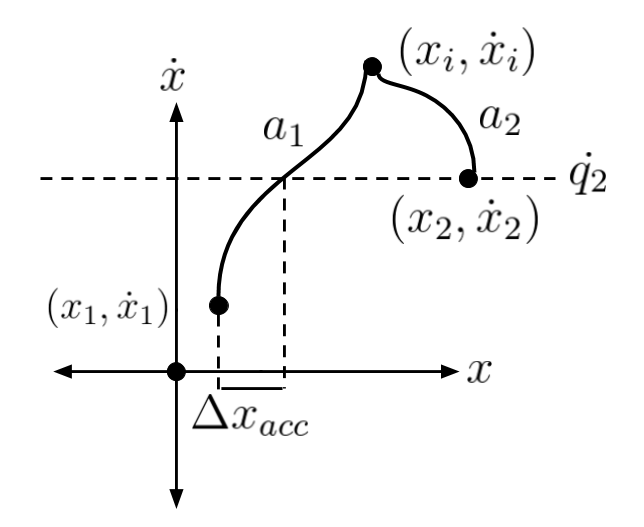
\includegraphics[width=0.3\textwidth]{fig/example_motion.png}
  \caption{
    \captionstyle
  	Example possible motion using the double-integrator minimum time model between start state $(x_1, \dot{x_1})$ and goal state $(x_2, \dot{x_2})$ through some intermediate state $(x_i, \dot{x_i})$.
  	}
   	\label{fig:sample_dimt}
\end{figure}

In order to find the minimum time, $T\left(x\right)$, of a motion like Fig. ~\ref{fig:sample_dimt}, we can examine the paths separately with one corresponding to a motion with acceleration $a_1$ from $\left(x_1, \dot{x}_1\right)$ to $\left(x_i, \dot{x}_i\right)$ and another corresponding to motion with acceleration $a_2$ from $\left(x_i, \dot{x}_i\right)$ to $\left(x_2, \dot{x}_2\right)$.

\ref{} shows that we can express total distance travelled in the joint space $x$ can be expressed in this way as:

\begin{equation}
x_2 - x_1 = d_{a_1} + d_{a_2}
\end{equation}
where $d_{a_1}$ is the distance travelled at max acceleration from the first path and $d_{a_2}$ is the distance travelled at max acceleration in the opposite direction.

Using simple constant acceleration equations we can express this in the form:

\begin{equation}
x_2 - x_1 = \left(\dot{x}_1 t_{a_1} + \frac{1}{2} a_1 t_{a_1}^2\right) + \left(\frac{\dot{x}_2^2 - \dot{x}_i^2}{2a_2}\right)
\end{equation}
where $t_{a_1}$ is the time it takes to make the path from $\left(x_1, \dot{x}_1\right)$ to $\left(x_i, \dot{x}_i\right)$ at acceleration $a_1$ and $t_{a_2}$ is the time it takes to make the path from $\left(x_i, \dot{x_i}\right)$ to $\left(x_2, \dot{x}_2\right)$ at acceleration $a_2$.

We can further expand the equation in order to put it into the canonical quadratic equation as follows:

\begin{equation}
a_1 t_{a_1}^2 + 2 \dot{x}_1 t_{a_1} + \frac{\dot{x}_2^2 - \dot{x}_1^2}{2a_2} - \left(x_2 - x_1\right) = 0
\end{equation}

Following ~\ref{} we solve a quadratic equation of the form $at^2+bt+c=0$ as follows:

$$
q = -\frac{1}{2}\left(b + \text{sign}\left(b\right)\sqrt{b^2 - 4ac}\right)
$$
$$
t_1 = \frac{q}{a}; \hspace{5mm} t_2 = \frac{c}{q}
$$
where $t_1$ and $t_2$ are the two solutions to the quadratic equation.

As we know, time must be positive and we are looking for minimum time. This leads to the fact that there is only one correct solution to the quadratic equation. Because of this, depending on the start and goal states, the sign of the acceleration on each path will change.

Again following ~\ref{}, we programatically solve for the sign of the sign of the acceleration by analysing the start and goal position. Fig. ~\ref{fig:sample_dimt} shows the determining term $\Delta x_{acc}$, which is the distance from $x_1$ to the point where $\dot{x} = \dot{x}_2$. 

And using constant acceleration equations with ~\ref{} again, we find that:

\begin{equation}
\Delta x_{acc} = \frac{1}{2} \left(\dot{x}_1 + \dot{x}_2\right) \frac{|\dot{x}_2 - \dot{x}_1|}{a_{max}}
\end{equation}

\begin{equation}
a_1 = - a_2 = \text{sign}\left(x_2 - x_2 - \Delta x_{acc}\right) a_{max}
\end{equation}

From these equations it shows a fundamental difference of a kinodynamic state space compared to a geometric state space. Because of this the minimum time path can vary in shape depending on the start and goal state. The consequence of this is that the shape of the informed subset can change dramatically depending on the start and goal state of the problem definition. Because of this, finding a closed form solution to sampling in the informed space is not feasible.
}

\ignore{
See Fig.~\ref{fig:informed_1d_di} for a visualization of the cost surface for a specific start and goal state for one degree of freedom (two dimensions $\left(x, \dot{x}\right)$). Lower costs are represented with cooler colors with warmer colors representing higher costs. One can see the minimum cost path from start to goal as the dark blue curve.
}

\begin{figure}[tb]
  \centering
  	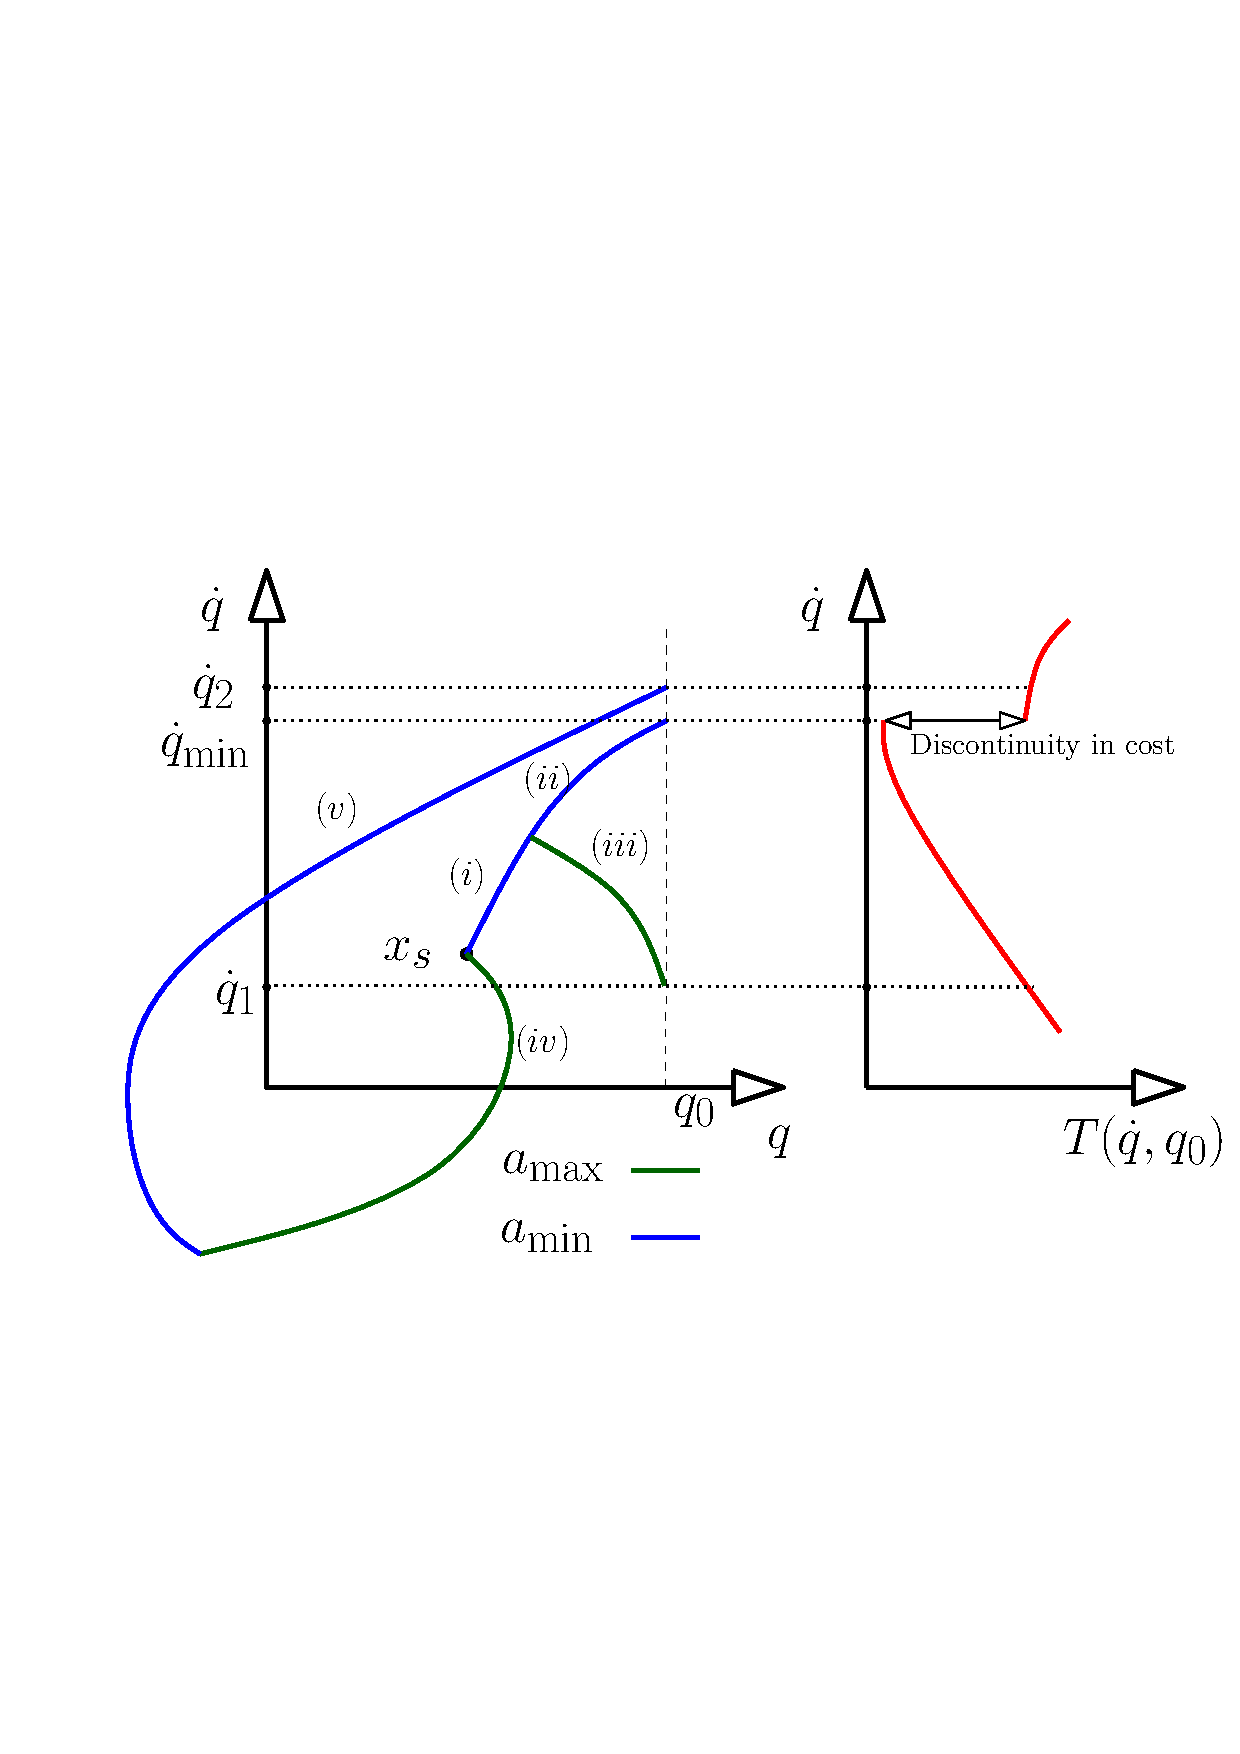
\includegraphics[height = 5.25cm ]{fig/cost_discontinuity.pdf}
  \caption{
    \captionstyle
  	Visualization of the discontinuity in the cost function of MTDI (right) related to the types of controls applied (left). 
  	Given state~$x_s$ and fixed position $q_0$, we depict the cost (time) as a function of the velocity~$\dot{q}$. 
  	The minimal cost is attained at $\dot{q}_{\min}$ by applying maximal acceleration (blue curves~$(i), (ii)$). 
  	To reach states such as~$\dot{q}_1$, where $\dot{q}_1 < \dot{q}_{\min}$ we need to apply maximal acceleration (curve~$(i)$) followed by minimal acceleration (green curve~$(iii)$), which result in a continuous increase in cost.
  	However, for states such as $\dot{q}_2$, where $\dot{q}_2 > \dot{q}_{\min}$, we need to apply minimal acceleration  followed by maximal acceleration (curves~$(iv), (v)$), which result in the discontinuity.
  	}
   	\label{fig:discont}
\end{figure}

\ignore{
\begin{figure}[tb]
  \centering
  	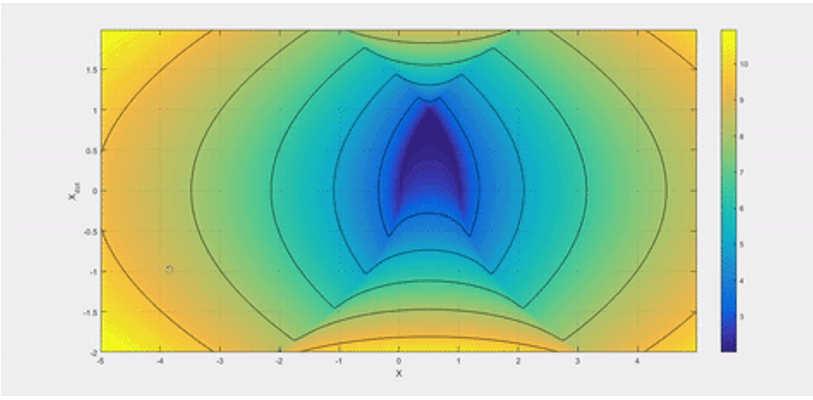
\includegraphics[height = 4.cm ]{fig/level_set.jpg}
  \caption{
    \captionstyle
  	Level sets for the case of minimal-time double integrator. A point $x = (q, \dot{q})$  denote the position and velocity of the robot while the color at $x$ denotes the cost to reach $x_t$ from $x_s$ subject to passing through the state $x$.
  	}
   	\label{fig:informed_1d_di}
	\vspace{-5.5mm}
\end{figure}

\begin{figure}[tb]
  \centering
  	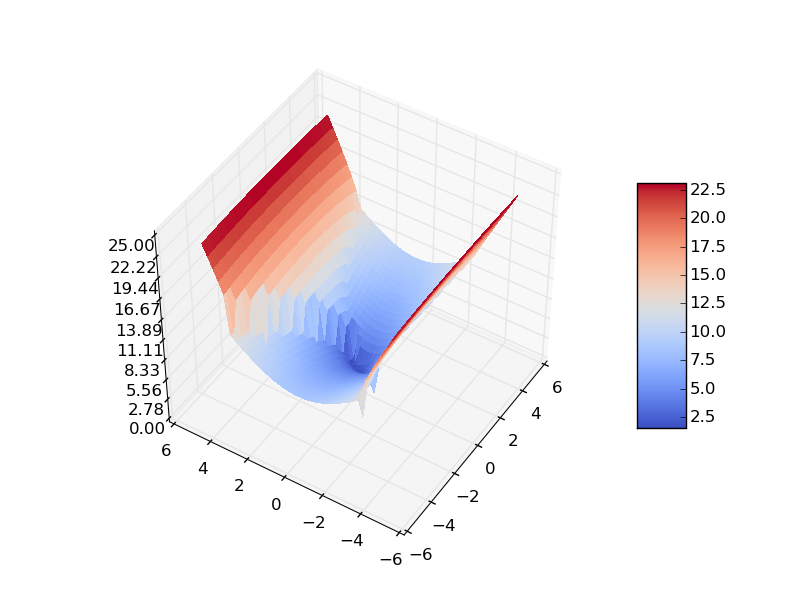
\includegraphics[width=0.5\textwidth]{fig/kino_space.png}
  \caption{
    \captionstyle
  	Side view of the cost surface for the case of minimal-time double integrator. The side view showcases the discontinuous nature of the cost surface.
  	}
   	\label{fig:cost_surface_1d}
%	\vspace{-5.5mm}
\end{figure}

See Fig.~\ref{fig:cost_surface_1d} for a side view of the cost surface for one degree of freedom ($\left(x, \dot{x}\right)$). One can see a key property of the cost surface that cause serious concerns is the discontinuous nature of the surface. As mentioned before, finding the minimum time problem amounts to solving a quadratic equation. Because the nature of this equation changes with the start and end goal, there is a curve in the input space that amounts to a switching surface that represents the boundary for the decision of the sign of $a_1$. This surface causes a discontinuous cost surface as shown in Fig. ~\ref{fig:cost_surface_1d}.
}

\section{MCMC-based Informed Sampling}
\label{sec:algorithm}

In this section we describe our approach to efficiently produce a sequence of samples in the informed set~\Cinf given a specific cost~$c_{\text{best}}$ of trajectory $x_{best}(t)$.
Our algorithm (see Alg.~\ref{alg:mcmc_informed_sampling}) starts by randomly sampling a state~$x_\text{rand} \in \calX$ (line~2).
This sample is used to produces a 
sample~$x_0 \in \partial\Cinf$ 
%sample~$x_\text{boundary} \in \partial\Cinf$ 
which lies (approximately) on the boundary of the informed set (Sec.~\ref{subsec:grad}) by applying Newton-Raphson method~\cite{RT06} (line~3).
Finally,~$x_0$ 
%use~$x_\text{boundary}$ 
is used (lines~4-6)
to initialize an MCMC algorithm which outputs a series of samples within \Cinf by constructing a Markov Chain.
This is done until some termination criterion is met and the entire process is repeated (Sec.~\ref{subsec:mcmc}). 
%Specifically, we chose to use HMC due to its favourable properties (see Sec.~\ref{sec:intro}). 
For a visualization of the approach, see Fig.~\ref{fig:alg}.

It is important to note that at each iteration, we will query our algorithm for one sample. However, this sample depends on the previous iterations of the algorithm which is why we describe it as a method to produce a sequence of samples.
Furthermore, the value~$c_{\text{best}}$ can decrease between consecutive iterations.
This will occur if the search algorithm that uses our sampler finds a path to the goal whose cost is lower than~$c_{\text{best}}$.

\os{mention that it is AO}

\begin{algorithm}[t]
	\begin{algorithmic}[1]
		\LOOP
			\STATE $x_{0} \leftarrow \texttt{sample\_in\_informed\_space}( method )$
			\WHILE {\texttt{MCMC\_continue\_chain()}}
			\STATE $x_{i} \leftarrow \texttt{MCMC\_sample} (x_{i-1}, c_{\text{best}})$
			\STATE \textbf{output} $x_{i}$
			\ENDWHILE
		\ENDLOOP 
%		\STATE $x_{\text{rand}} \leftarrow \texttt{sample\_uniform(\calX)}$
%%		\STATE $x_{\text{boundary}} 
%		\STATE $x_{0} 
%		 \leftarrow
%		 \texttt{newton\_raphson}(x_{\text{rand}}, c_{\text{best}})$ ; \hspace{3mm} $i\leftarrow 0$
%%		\STATE $x_{0} \leftarrow x_{\text{boundary}}$
%		\WHILE {\texttt{MCMC\_continue\_chain()}}
%			\STATE $x_{i} \leftarrow \texttt{MCMC} (x_{i-1}, c_{\text{best}})$; \hspace{3mm} $i\leftarrow i+1$
%			\STATE \textbf{output} $x_{i}$
%		\ENDWHILE		
%		\FOR {$i = 1$ to $N$}
%			\STATE $x_{i} \leftarrow \texttt{MCMC} (x_{i-1}, c_{\text{best}})$
%			\STATE \textbf{output} $x_{i}$
%		\ENDFOR
   	\end{algorithmic}
	\caption{MCMC-based Informed Sampling $(c_{\text{best}})$}
	\label{alg:mcmc_informed_sampling}	
\end{algorithm}

\subsection{Sampling the boundary of \Cinf}
\label{subsec:grad}
We can use either of the following two approaches to sample points in the informed space:
\subsubsection{Newton-Raphson Method}
In theory, MCMC methods converge to the desired distribution regardless of the initial sample used to seed the chain.
In our setting, the probability distribution~\Pinf is defined by having all points in \Cinf distributed uniformly
while 
the probability of sampling any configuration $x \in \calX \setminus \Cinf$ is zero.
A common practice to avoid starting biases in MCMC-type algorithm is to discard an initial set of samples (a process referred to as ``burn-in'')~\cite{ADDJ03}. 

In our setting, we are only interested in points in~\Cinf, thus we can start the Markov Chain in~\Cinf and avoid this burn-in stage. 
To do so we apply  Newton-Raphson's method to obtain a sample on $\partial \Cinf$. 
However, our cost function is not necessarily continuous (see Sec.~\ref{sec:mtdi}), thus if no sample was produced on $\partial \Cinf$ after a predefined number of steps, we restart the algorithm using a different random state~$x_\text{rand}$
(see also Sec.~\ref{subsec:mcmc}).

\subsubsection{Previous-Trajectory Method}


\subsection{Sampling the interior of \Cinf via MCMC}
\label{subsec:mcmc}

Our approach is general and can be applied to any MCMC algorithm (see Sec.~\ref{sec:related_work}).
We demonstrate how to instantiate it with two different algorithms: 
Hit and Run and Metropolis-Hastings.

For each algorithm, 
we describe how it is used to 
(i)~sample points 
(\texttt{MCMC\_sample, line 5})
and 
(ii)~decide if to continue sampling along the Markov Chain or to restart the entire process 
(\texttt{MCMC\_continue\_chain, line 4}).
 
\subsubsection{Hit and Run}
\begin{algorithm}[t]
	\begin{algorithmic}[1]
		\STATE $d \leftarrow$ \texttt{sample\_random\_direction}$()$
		\STATE $ L(\lambda) = \{  x \mid x = x_{i-1} + \lambda d_i \} $
		\STATE $ \lambda^{+} \leftarrow \sup L(\lambda) $; 
				\hspace{3mm} 
			   $ \lambda^{-} \leftarrow \inf L(\lambda) $
			   
		\LOOP


		\STATE $ \lambda' \leftarrow$ \texttt{sample\_random}$ (\lambda^{-} , \lambda^{+})$
		\STATE $ x_{i} \leftarrow x_{i-1} + \lambda'_{i} d_i $
		
		\IF{ \textsc{Cost}($ x_{i} $) $ < c_{\text{best}} $ }
		  \RETURN $ x_{i}$
		\ENDIF


		\IF{ $ \lambda' > 0 $ }
			\STATE $ \lambda^{+} \leftarrow \lambda' $
		\ELSE
			\STATE $ \lambda^{-} \leftarrow \lambda'$
		\ENDIF
		
		\ENDLOOP
  	\end{algorithmic}
	\caption{Hit-And-Run MCMC $(x_{i-1}, c_{\text{best}})$}
	\label{alg:hit_and_run_mcmc}	
\end{algorithm}

We use the Accelerated Hit and Run algorithm \cite{KSZ11}, described in Alg.~\ref{alg:hit_and_run_mcmc} that produces a series of samples $x_0, \ldots$.
Given the previous sample~$x_{i-1}$ it first  samples a random direction on the unit sphere (line 1).
This induces a line~$L(\lambda)$ passing through~$x_{i-1}$  in the direction sampled (line 2) parametrized by a scalar~$\lambda$.
We obtain upper and lower bounds on $\lambda$ (line 3) that are problem dependant. For example, if we have box constraints on joint limits of the robot and on maximum velocity, then bounds are given by $\lambda^{+} = -\lambda^{-} = l_{diag}$; where $l_{diag}$ is the length of the longest diagonal of the box.
We then sample a point along~$L(\lambda)$ by sampling a scalar~$\lambda'$ within our bounds (line 5).
This defines a point~$x_{i}$ which is a candidate for the next sample along the Markov Chain (line 6).
We then check if the point lies in the informed set (line 7) and if it does we return it.
If not, we update our bounds (lines~9-12) and repeat the process.
The algorithm can be viewed as an efficient method that performs rejection sampling along a one-dimensional line passing through the previous sample parametrized by $\lambda$.

For this algorithm, we continue sampling along the Markov Chain until either 
(i)~the difference between the lower and upper bounds ($\lambda^-$ and $\lambda^+)$ 
that define our sampling domain is below a predefined threshold or
(ii)~a predefined number of samples was exceeded.

\os{Mention that we do not need convexity}

\begin{algorithm}[t]
	\begin{algorithmic}[1]
	    \LOOP
		\STATE $ x'_{i} \leftarrow \texttt{sample\_normal}(x_{i-1},\Sigma) $ 
		\label{start}
		\IF{ $ x'_{i} \leftarrow$ \texttt{sample\_random}$ (0.0 , 1.0) >  \pi( x'_{i} ) / \pi( x_{i} ) $  }
		\STATE x
 		\ENDIF
		\IF{ \textsc{Cost}($ x_{i} $) $ < c_{\text{best}} $  }
		  \RETURN $x_{i}$
		\ENDIF 
		\ENDLOOP
	\end{algorithmic}
	\caption{Metropolis-Hastings MCMC $(x_{i-1}, c_{\text{best}})$}
	\label{alg:mh_mcmc}	
\end{algorithm}

\begin{algorithm}[t]
	\begin{algorithmic}[1]
	\IF{ $method = \texttt{Newton-Rapson}$  }
		\STATE $x_{\text{rand}} \leftarrow \texttt{sample\_uniform(\calX)}$
		\STATE $x_{0} \leftarrow \texttt{newton\_raphson}(x_{\text{rand}}, c_{\text{best}})$ ; \hspace{3mm} $i\leftarrow 0$
	\ELSIF{ $method = \texttt{Previous-Trajectory}$ }
	    \STATE $t_{rand} \leftarrow \texttt{sample\_random\_time()}$
	    \STATE $x_{0} \leftarrow x_{best}(t_{rand})$
	\ENDIF
	\RETURN $x_0$
	\end{algorithmic}
	\caption{sample\_in\_informed\_space$(method, c_{best})$}
	\label{alg:sample_inf}	
\end{algorithm}

\subsubsection{Metropolis-Hasting}

The Metropolis-Hastings algorithm, describe in Alg.~\ref{alg:mh_mcmc}, also uses rejection sampling around the previously generated sample to propose the next sample of the Markov Chain.
While the general algorithm is slightly more complex, for our setting it can be described as follows:
We generate a new sample $ x_{i}$ around the previous sample $ x_{i-1}$ using a Gaussian distribution (line~1).
We then check if the point lies in the informed set (lines 2-5) and if it does we return it.
If not, we return the previous sample.
%
For this algorithm, we continue sampling along the Markov Chain as long as new samples are produced.


\section{Evaluation}
\label{sec:eval}

% \subsection{Uniformity}

% (Give a set of parameters)
% We firstly need to propose a way of measuring uniformity.
% Then we can apply it to compare MCMC approach with rejection sampling and hierarchical rejection sampling.
% We are interested with
% \begin{itemize}
% 	\item asymptotic behavior (assumption: MCMC converge to a close uniformity)
% 	\item convergence rate (assumption: MCMC converge faster)
% \end{itemize}

We evaluate the performance of proposed MCMC methods by comparing four types of samplers, which are rejection sampler (RS), hierarchical rejection sampler (HRS), Metropolis-Hastings sampler (MHS), and Hit-and-run sampler (HNR).
We use different samplers to generate a fixed number of samples in different informed sets to check the sampling efficiency, especially when the sampling is harder (in a small informed set).
We then evaluate how the samplers works with informed RRT*~\cite{GSB14}, which reflect the quality of samples in an informed set.

\subsection{Sampling Efficiency}

Fig. \ref{fig:sampling_efficiency} shows the log plot of the average time taken to generate one sample in the informed space vs. informed set volume ratio, i.e. the ratio of the volume of informed space to the volume of entire state space for 5000 samples. 
The informed set volume ratio is approximated by the ratio of the number of accepted to the total number samples obtained while running rejection sampling. Efficiency of rejection sampling based methods is very low for high dimesions because this ratio decreases exponentially w.r.t the dimension of the space due to the curse of dimensionality. 
The Fig. \ref{fig:sampling_efficiency} shows that MCMC and Hit\&Run have a better sampling efficiency compared to HRS and RS with decrease in informed set ratio or increase in dimensions. 
Figure \ref{fig:sampling_efficiency:levelset} shows how the informed set volume ratio decreases as the level set cost $ c_{best} $ becomes smaller in problems of different dimensions.
In a higher dimension, the informed set volume ratio falls much more quickly as the level set cost $ c_{best} $ decreases in planning process, as new better solutions are kept being found.

\begin{figure}[t!]
	\centering
	\begin{subfigure}[b]{0.78\linewidth}
		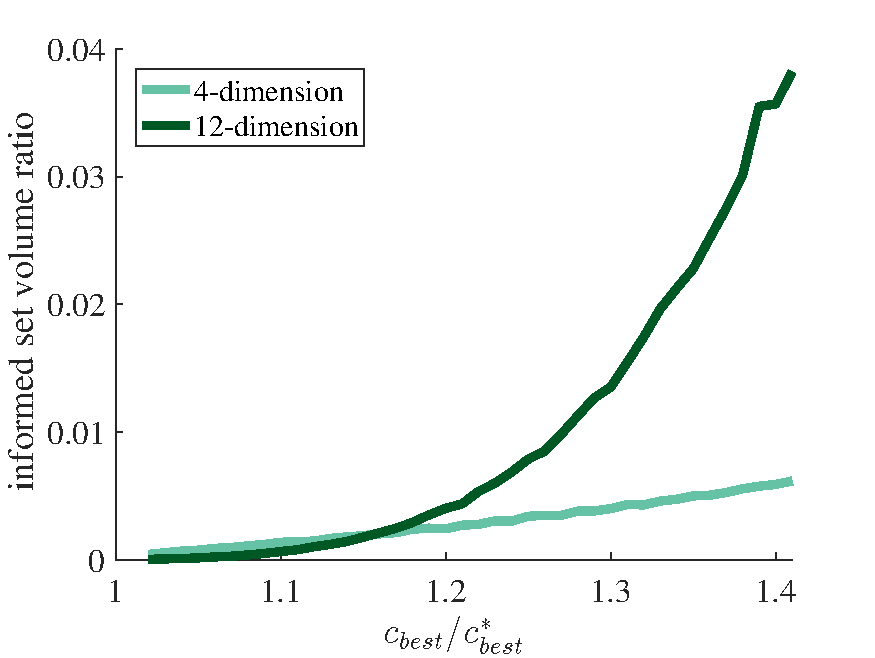
\includegraphics[width=\linewidth]{fig/sampling_efficiency/levelset}
		\caption{2DoF - 4D. TODO:Time per sample vs level set}
		\label{fig:sampling_efficiency:levelset}
	\end{subfigure}
	%\begin{subfigure}[b]{0.48\linewidth}
	%	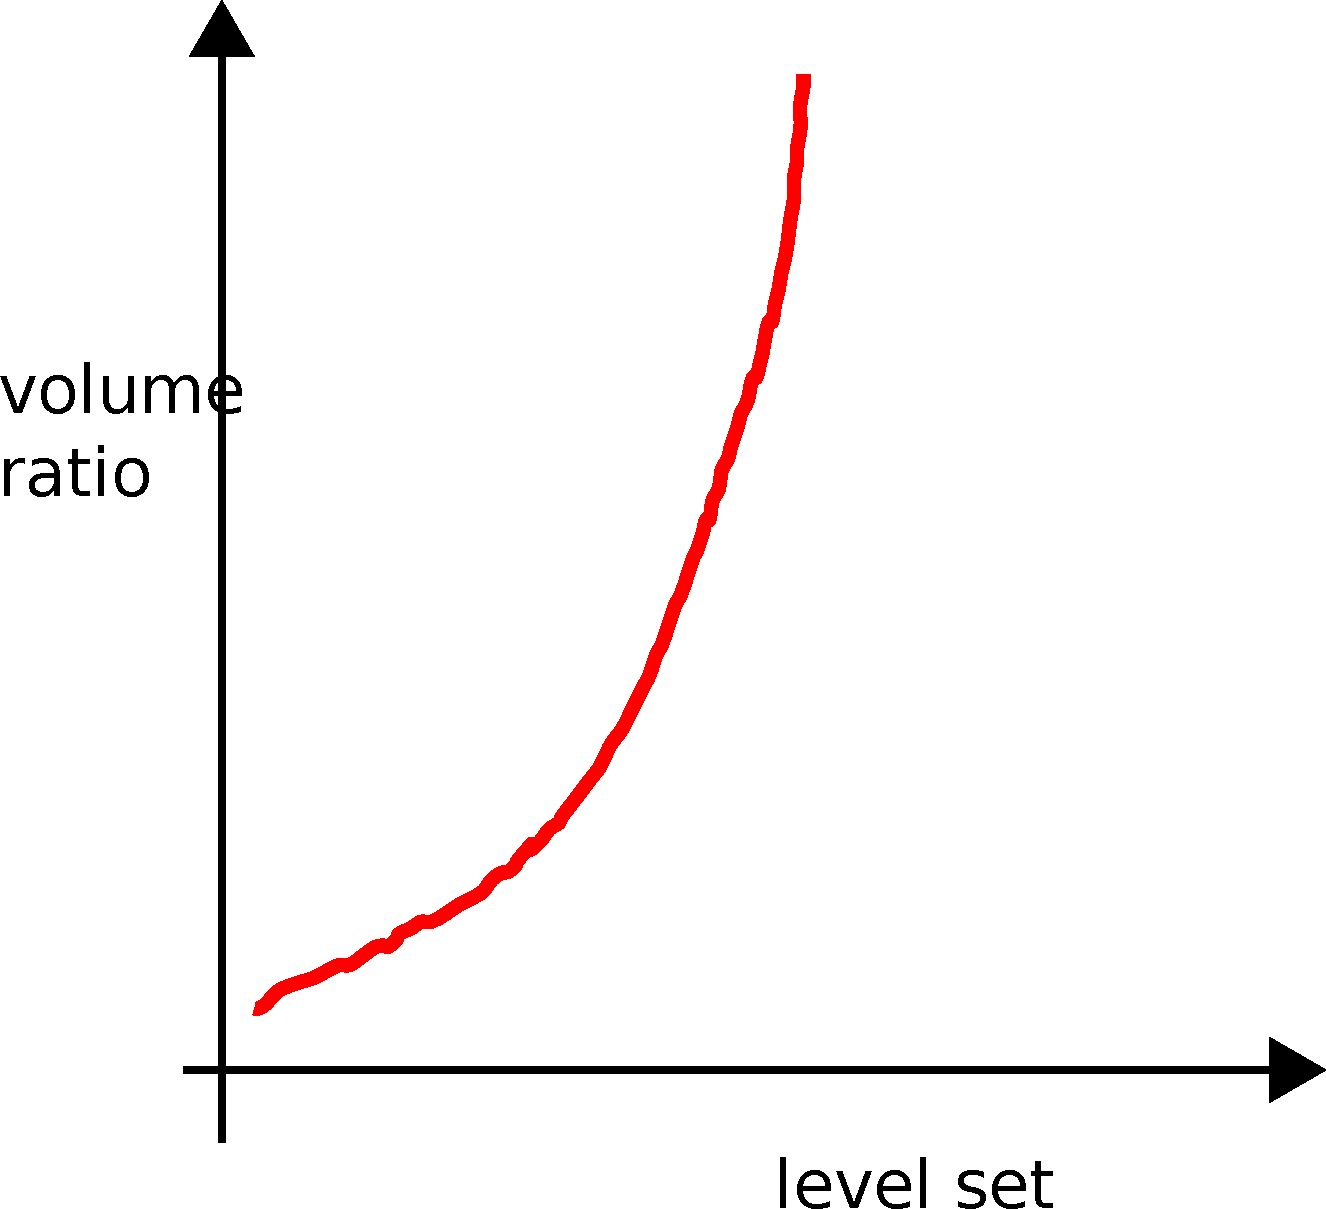
\includegraphics[width=\linewidth]{fig/sampling_efficiency/levelset_6d}
	%	\caption{6DoF - 12D. TODO:Time per sample vs level set}
	%	\label{fig:sampling_efficiency:6d}
	%\end{subfigure}
	 \\
	\begin{subfigure}[b]{0.78\linewidth}
		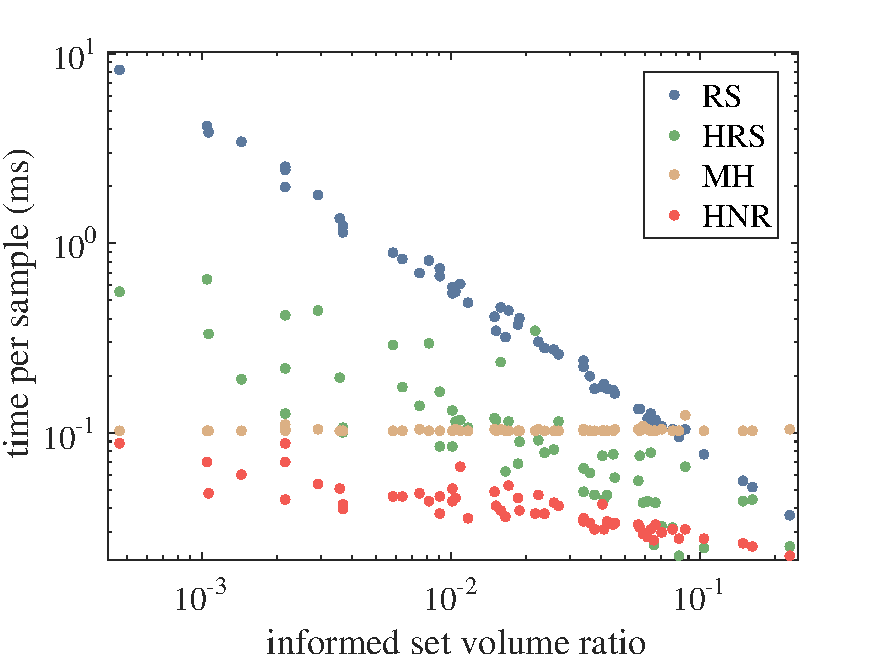
\includegraphics[width=\linewidth]{fig/sampling_efficiency/sample_efficiency_2d}
		\caption{2DoF - 4D TODO: rescale x axis}
		\label{fig:sampling_efficiency:2d}
	\end{subfigure}
% 	\begin{subfigure}[b]{0.32\textwidth}
% 		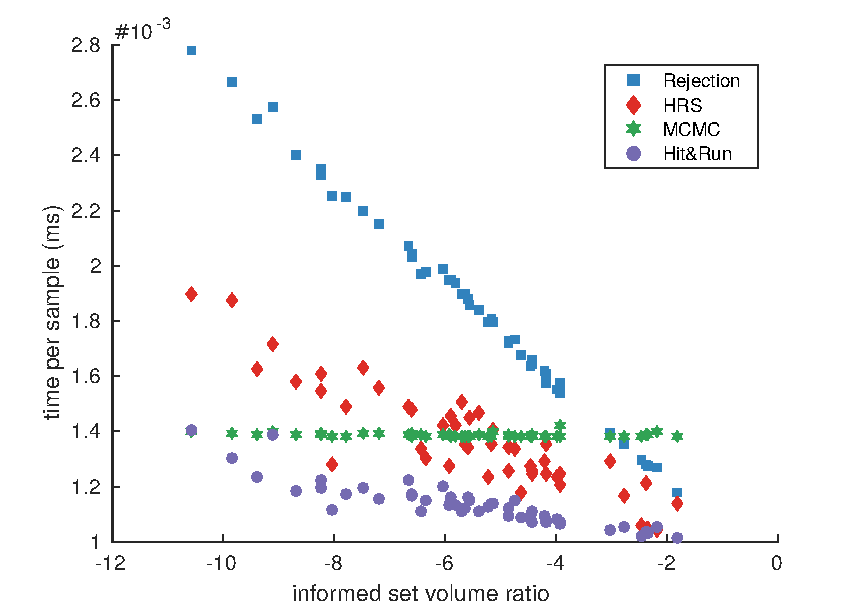
\includegraphics[width=\linewidth]{fig/sampling_efficiency/sample_efficiency_3d}
% 		\caption{3DoF - 6D}
% 		\label{fig:sampling_efficiency:3d}
% 	\end{subfigure}	
	\begin{subfigure}[b]{0.78\linewidth}
		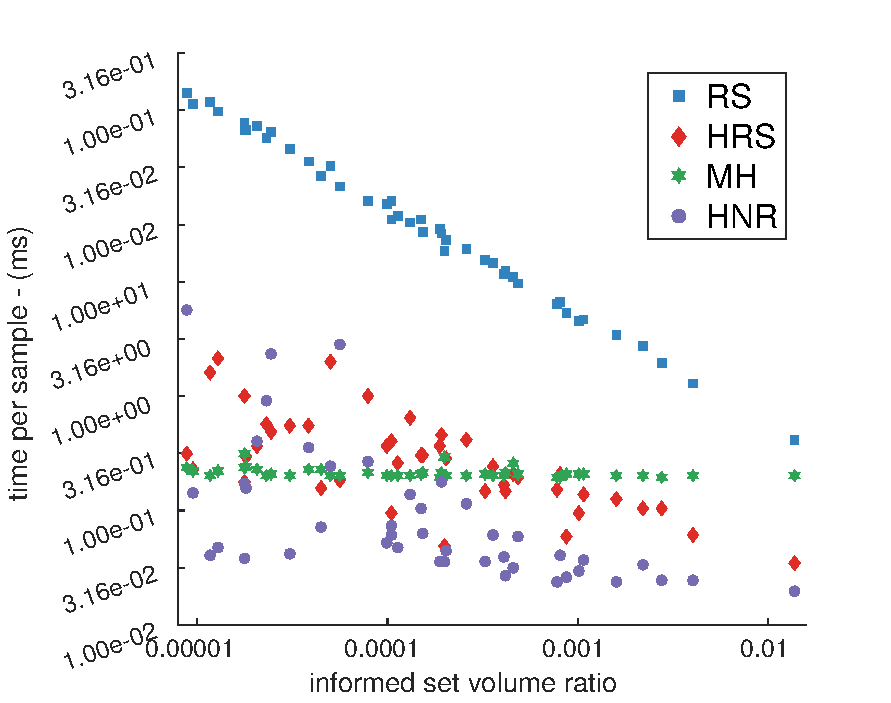
\includegraphics[width=\linewidth]{fig/sampling_efficiency/sample_efficiency_6d}
		\caption{6DoF - 12D. TODO: rescale x axis}
		\label{fig:sampling_efficiency:6d}
	\end{subfigure}
	\caption{\captionstyle Sampling efficiency of different sampling methods}
	\label{fig:sampling_efficiency}
\end{figure} 
vantage of sampling a near state.
Both the per-sampling time of HRS 
It is noticeable that both x axis and y axis are converted by $ \log_{10} () $ in Figure~\ref{fig:sampling_efficiency:2d} and Figure~\ref{fig:sampling_efficiency:6d}.
This reserves the linearity of the data from rejection sampler, but also scales the difference in a smaller range for comparison.
Keep in mind that the differences in unit (ms) are much bigger.
\dy{TODO: change MCMC to MH (Metropolis Hasting) in the plots}
Metropolis-Hasting shows consistent performance when the informed set volume ratio is decreased, because it takes the adand HNR increases with the decrease of the informed set volume ratio. 
When informed set volume ratio is relatively high, it is easy to generate qualified samples.
All the samplers have close performances.
RS and HRS can be the most efficient because of its simple design.
But when problems get harder, HNR outperforms HRS significantly.

\os{Explain why MCMC is flat, mention strawman approach}

\subsection{Planning Efficiency}

The quality of samples determines the efficiency of resulting planning algorithms.
To evaluate how the samplers impact the planning efficiency, we run the samplers with the informed RRT* planner~\cite{GSB14} on three different problems described below and shown in Fig. \ref{fig:problems}. 
For each problem the start and goal states (positions and velocities) are known in the joint space.

\subsubsection{Problem 1: 3 DoF Planar Manipulator}

Problem 1 is a 3 DoF manipulator that moves on a plane, which results in a 6 dimension space.
The position boundary of each join is $ [ - \pi , \pi ] $, the velocity boundary is $ [-10, 10] $, and the acceleration is $ 1 $.
Figure~\ref{fig:planning_efficiency:3dof:example} shows a few steps of a planned path.

\subsubsection{Problem 2: 6 DoF Snake Arm}

Problem 2 is a 6 DoF snake arm that moves in a 3D workspace, which results in a 12 dimension space.
The position boundary of each join is $ [ - \pi , \pi ] $, the velocity boundary is $ [-10, 10] $, and the acceleration is $ 1 $.
Figure~\ref{fig:planning_efficiency:6dof:example} shows a few steps of a planned path.

\subsubsection{Problem 3: 7 DoF HERB}

Problem 3 is a 7 DoF Barrett WAM arm of HERB that moves in a 3D workspace, which results in a 14 dimension space.
The position boundaries of 7 joints of the arm are $  [0.541593 , 5.74159] $, $  [-2 , 2] $, $ [-2.8 , 2.8] $, $ [-0.9 , 3.1] $, $ [-4.76 , 1.24] $, $ [-1.6 , 1.6] $ and $ [-3 , 3] $.
The velocity boundary of 7 joints of the arm are $ [-0.75 , 0.75] $, $ [-0.75 , 0.75] $, $ [-2 , 2] $, $ [-2 , 2] $, $ [-2.5 , 2.5] $, $ [-2.5 , 2.5] $ and $ [-2.5 , 2.5] $.
The accelerations of all the joints are set to $ 1 $.
Figure~\ref{fig:planning_efficiency:herb:example} shows a few steps of a planned path.

\begin{figure*}[t!]
	\centering
	\begin{subfigure}[b]{\textwidth}
	    \centering
		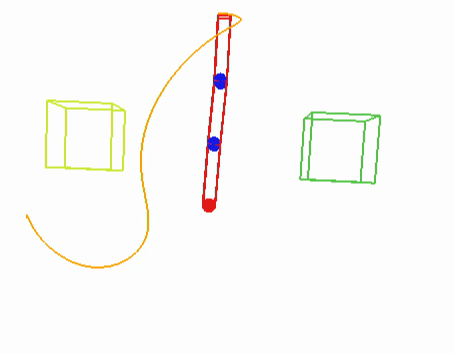
\includegraphics[height=2.45cm]{fig/planning_efficiency/3dof_1}
		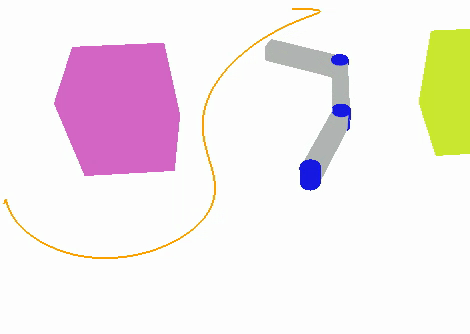
\includegraphics[height=2.45cm]{fig/planning_efficiency/3dof_2}
		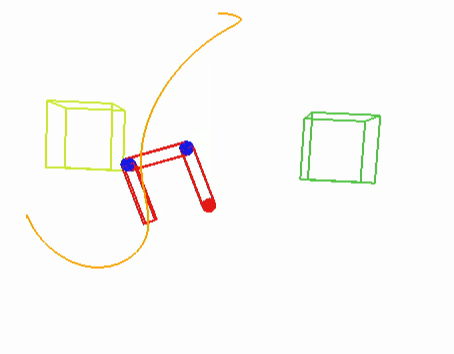
\includegraphics[height=2.45cm]{fig/planning_efficiency/3dof_3}
		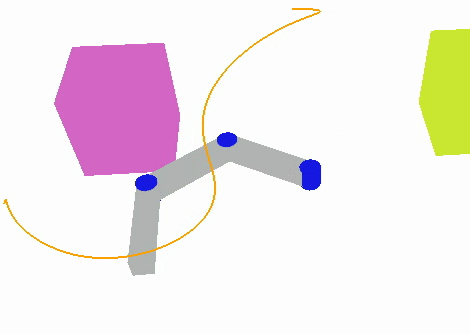
\includegraphics[height=2.45cm]{fig/planning_efficiency/3dof_4}
		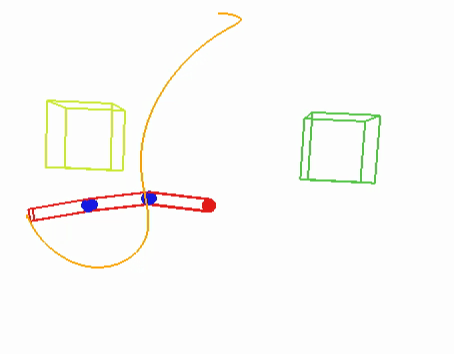
\includegraphics[height=2.45cm]{fig/planning_efficiency/3dof_5}
		\caption{3DOF planar}
		\label{fig:planning_efficiency:3dof:example}
	\end{subfigure}
	\begin{subfigure}[b]{\textwidth}
	    \centering
		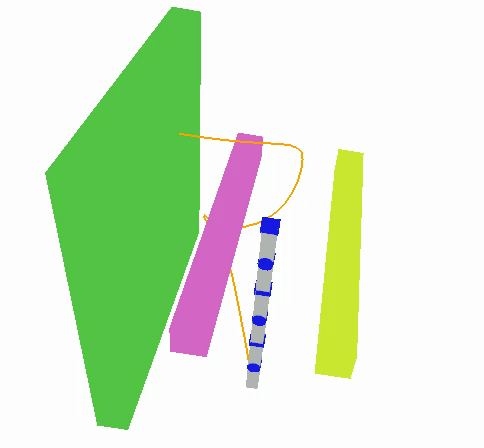
\includegraphics[height=3cm]{fig/planning_efficiency/6dof_1}
		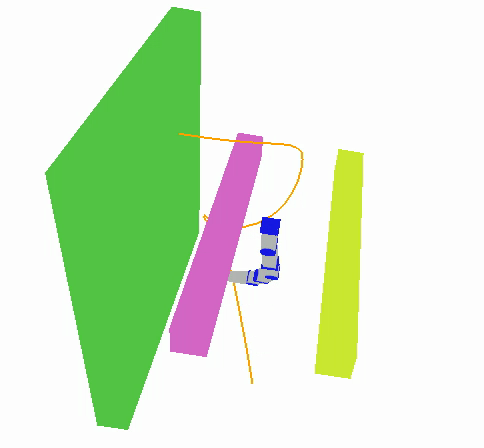
\includegraphics[height=3cm]{fig/planning_efficiency/6dof_2}
		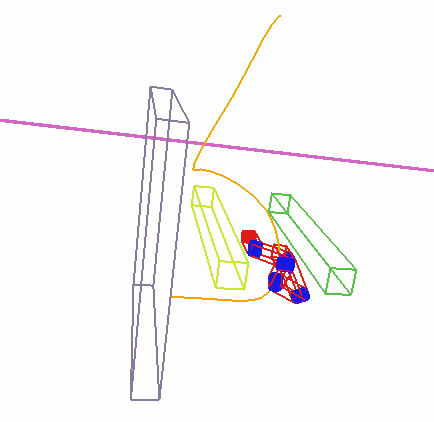
\includegraphics[height=3cm]{fig/planning_efficiency/6dof_3}
		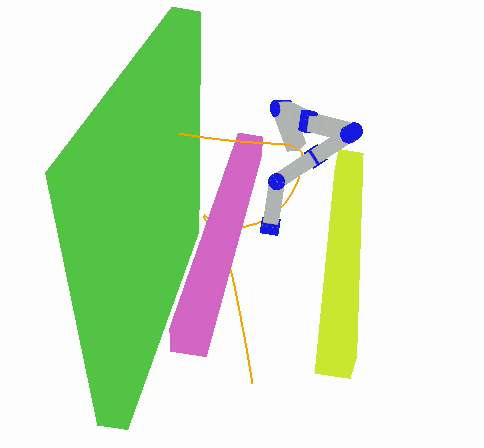
\includegraphics[height=3cm]{fig/planning_efficiency/6dof_4}
		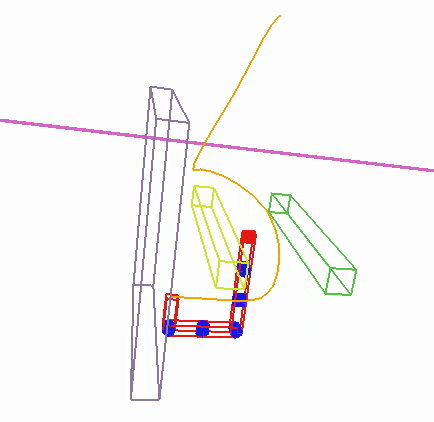
\includegraphics[height=3cm]{fig/planning_efficiency/6dof_5}
		\caption{6DOF snake}
		\label{fig:planning_efficiency:6dof:example}
	\end{subfigure}
	\begin{subfigure}[b]{\textwidth}
    \centering
    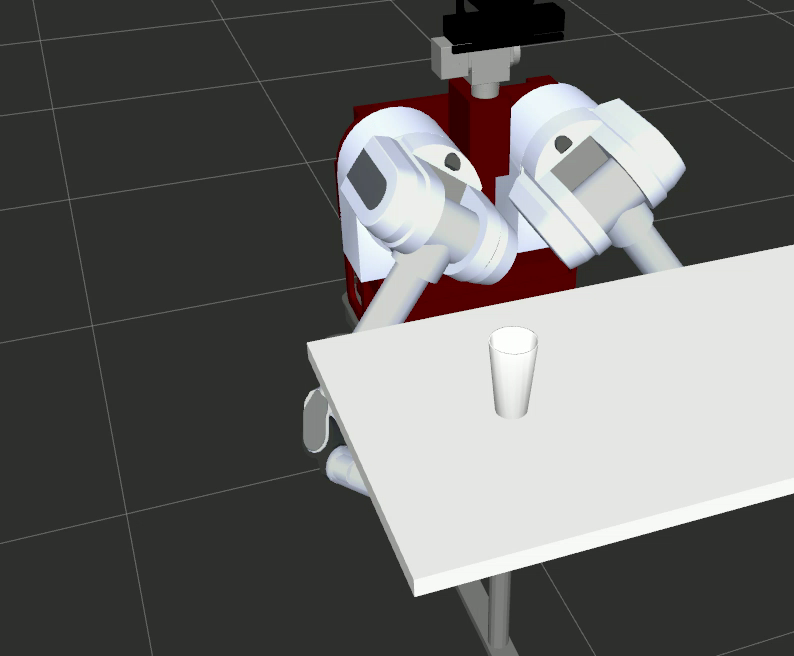
\includegraphics[height=2.7cm]{fig/planning_efficiency/herb_batting_1}
    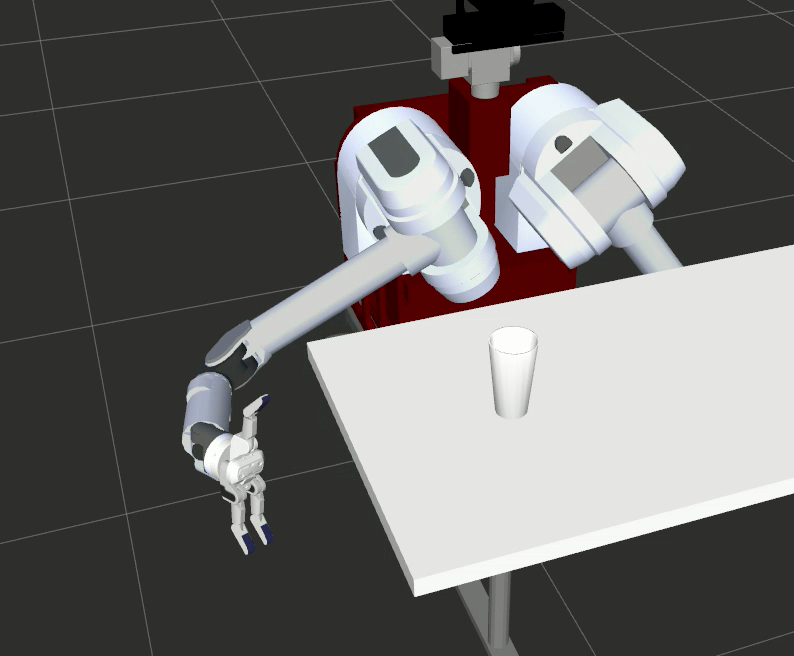
\includegraphics[height=2.7cm]{fig/planning_efficiency/herb_batting_2}
    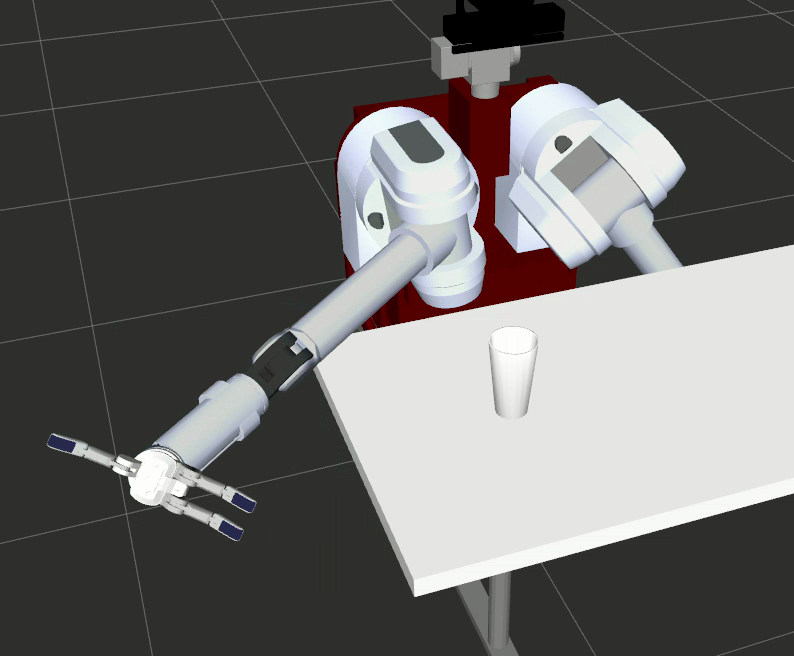
\includegraphics[height=2.7cm]{fig/planning_efficiency/herb_batting_3}
    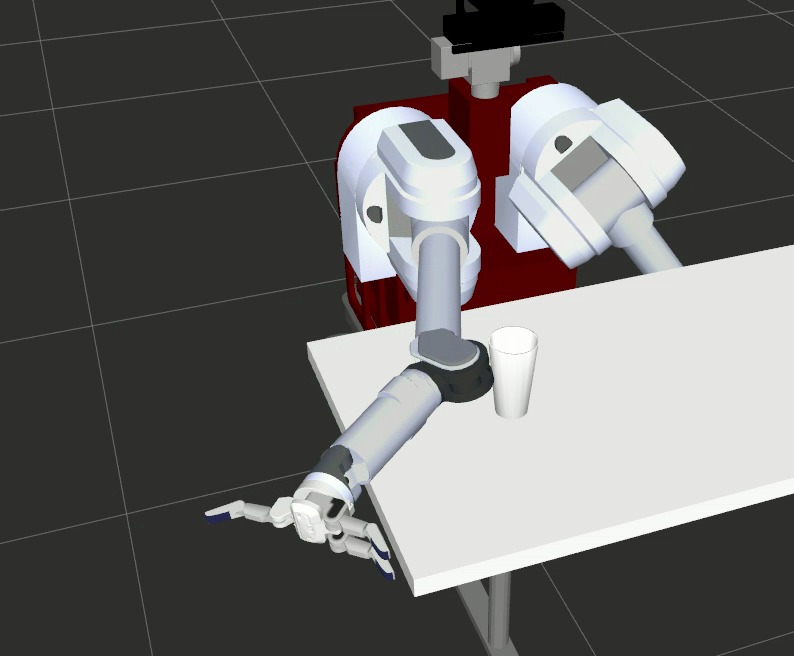
\includegraphics[height=2.7cm]{fig/planning_efficiency/herb_batting_4}
    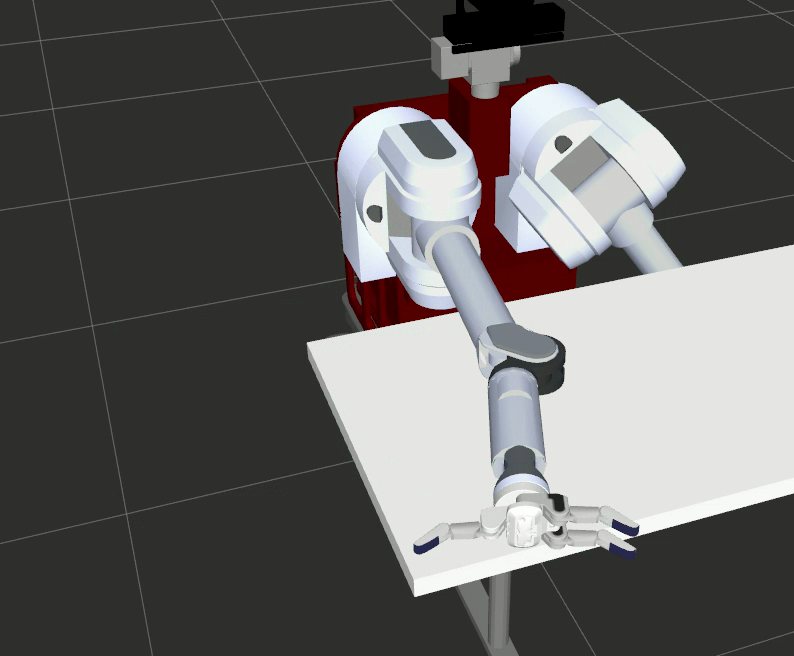
\includegraphics[height=2.7cm]{fig/planning_efficiency/herb_batting_5}
	\caption{HERB}
	\label{fig:planning_efficiency:herb:example}
	\end{subfigure}
	\caption{Test problems to evaluate planning efficiency. TODO: Add herb and update figures}
	\label{fig:problems}
\end{figure*} 


\begin{figure*}[t!]
	\centering
	\begin{subfigure}[b]{0.32\textwidth}
		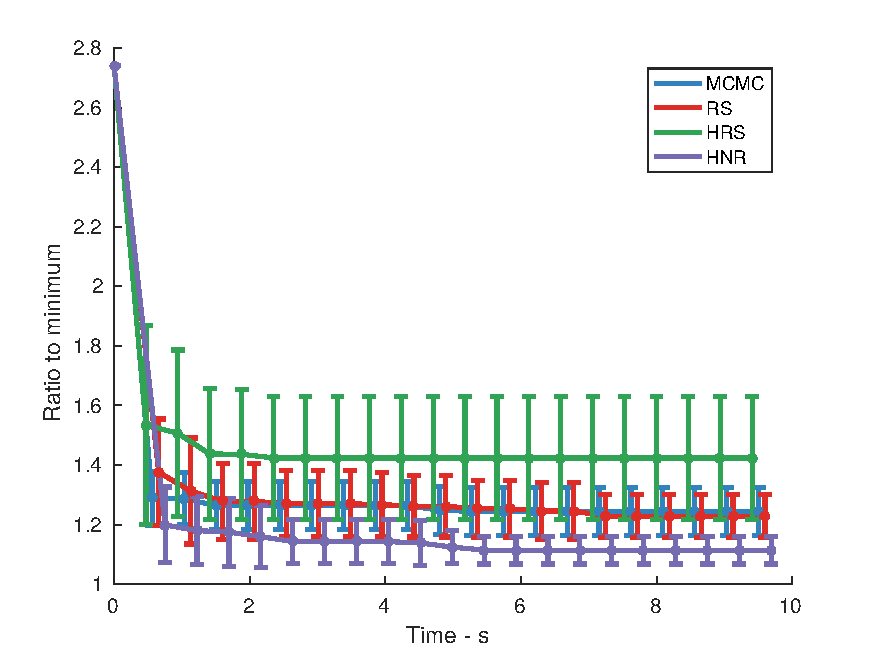
\includegraphics[width=\linewidth]{fig/planning_efficiency/3dof_general}
		\caption{\captionstyle Planning Efficiency for Problem 1: 3 DoF Manipulator}
		\label{fig:planning_efficiency:3dof:general}
	\end{subfigure}	
	\begin{subfigure}[b]{0.32\textwidth}
		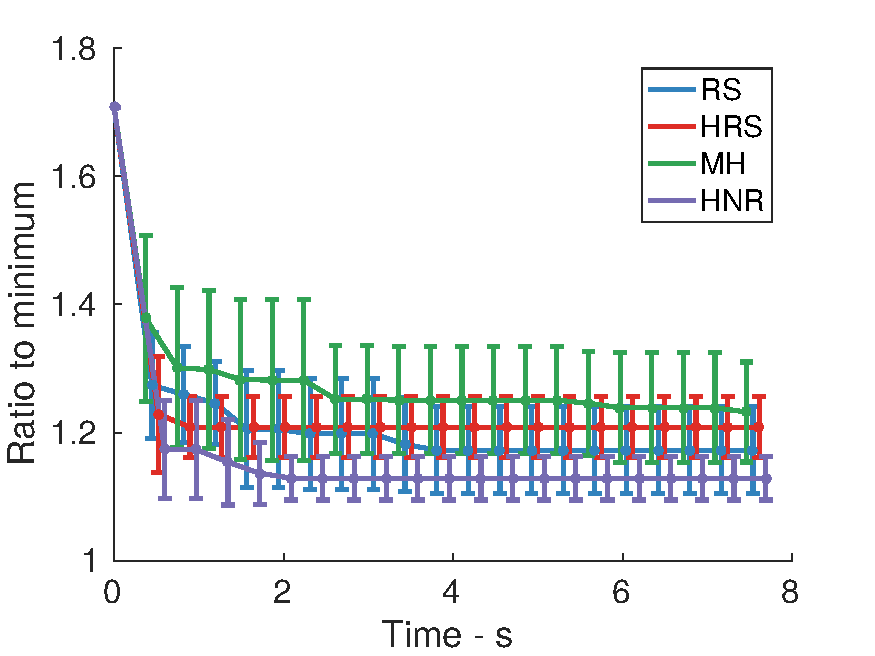
\includegraphics[width=\linewidth]{fig/planning_efficiency/6dof_hammering}
		\caption{\captionstyle Planning Efficiency for Problem 2: 6DoF Hammering Task}
		\label{fig:planning_efficiency:6dof:hammering}
	\end{subfigure}
	\begin{subfigure}[b]{0.32\textwidth}
	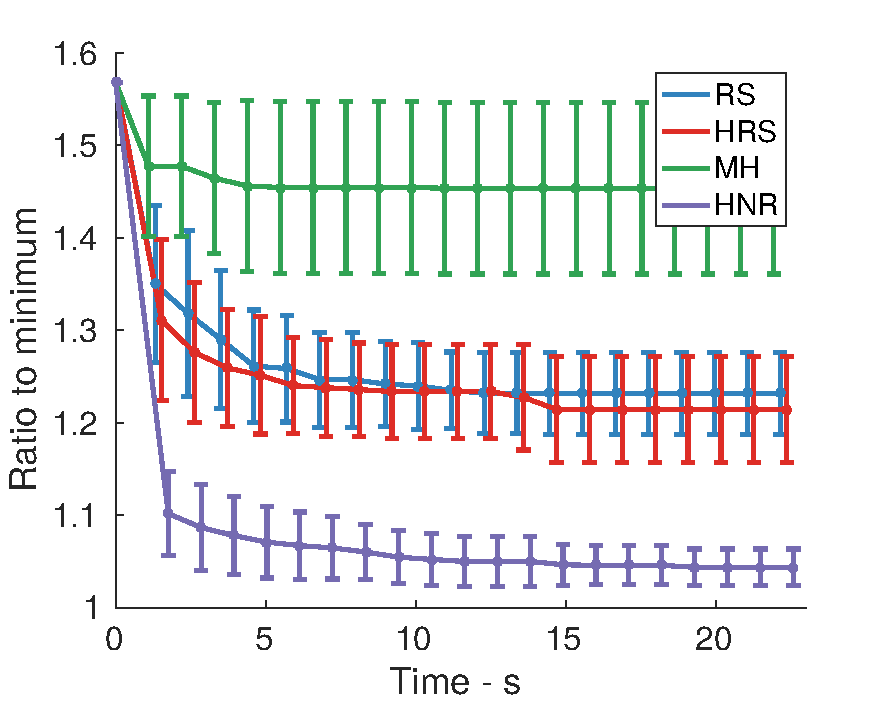
\includegraphics[width=\linewidth]{fig/planning_efficiency/herb_batting_efficiency}
	\caption{\captionstyle Planning Efficiency for Problem 3: 7DoF HERB Batting Task}
	\label{fig:planning_efficiency:herb:batting}
    \end{subfigure}
	\caption{Planning Efficiency}
	\label{fig:planning_efficiency}
\end{figure*} 

\dy{TODO: add a plot that shows the increases of samples}

MHS shows the worst performance in Figure~\ref{fig:planning_efficiency:3dof:general}, \ref{fig:planning_efficiency:6dof:hammering} and \ref{fig:planning_efficiency:herb:batting}.
Though theoretically samples converge to a target distribution, the samples could be either too correlated for exploration purpose in planning.
If the variance of transition distribution is too high, it will then move out of the informed set too frequently, and takes longer to converge.
Ideally we want to have markov chains are less correlated but moves in informed sets.

HNR shows close performance with RS and HRS in a 6-dimension space, as in Figure~\ref{fig:planning_efficiency:3dof:general}.
But in higher dimension performance, the advantage of HNR in sampling efficiency is shown.
In Figure~\ref{fig:planning_efficiency:6dof:hammering} and \ref{fig:planning_efficiency:herb:batting}, the cost of current best solution by planners with HNR sampler converge significantly faster.

\section{Conclusion}
\os{Discuss param tuning, we did nothing + there is a wealth of literature}

\os{use with BIT*, challenge - distance function is not a metric}



The Met

What MCMC algorithm is the best to use?

Parameter tuning

Application to different state spaces

Parallel chains

estimating volume of informed space




%%%%%%%%%%%%%%%%%%%%%%%%%%%%%%%%%%%%%%%%%%%%%%%%%%%%%%%%%%%%%%%%%%%%%%%%%%%%%%%%

\bibliography{bibliography}
\bibliographystyle{IEEEtran}
%\bibliography{IEEEabrv,bibliography}


\end{document}
